\textcolor{red}{endrullis: 
SPO: replacement in arbitrary context (drops all dangling edges)\\
SqPO : deterministic non-linear rewriting;\\
AGREEE: deterministic non-linear rewriting with a filtering mechanism;
In these approaches rules are applicable in any context: 1) no control over the embedding (edges incident to the pattern; 2) destructive:dangling edges will be dropped
}

\section{Pushout and pullback}
    \label{sec:category_theory}
    \begin{definition}[Category~\cite{pierce1991basic,barr1990category}]
    \label{def:cat}
    A \textbf{category} is an unlabeled graph \( C \) together with a total function \( u : C_0 \to C_1 \) and a partial function \( \star: C_1 \times C_1 \to C_1 \) such that 
        (i) for all edges \( f:X \to Y \) and \( g:Y \to Z \), the edge \( f \star g :X \to Z \) is defined; 
        (ii) for every node \( X \), \( u(X) \) is an edge from \( X \) to \( X \);
        (iii) for every \( f:X \to Y \), we have \(u(X) \star f = f = f \star u(Y)\);
        (iv) for all edges \( f \), \( g \) and \(h\), we have \( (f \star g) \star h = f \star (g \star h) \) whenever either side is defined.
    Edges are called \textbf{morphisms}. The function $\star$ is called \textbf{composition}. For all \( X \in C_0 \), the edge \( u(X) \) is denoted \( \operatorname{id}_X \) and is called the \textbf{identity} of the object \( X \).
    % \( C \) is called the \textbf{underlying graph} of the category \( \mathcal{C} \).
\end{definition} 

% cat notation * 
\begin{notation}
    The composition of morphisms \( f : X \to Y \) and \( g : Y \to Z \) is written in diagrammatic order as \( f \star g \), rather than in functional order \( g \circ f \). 
    % The advantage is that, when reading from left to right, the morphisms appear in the same order as in the corresponding diagram, making the notation more intuitive for visual reasoning.
\end{notation}  

\begin{definition}[Monomorphism~\cite{pierce1991basic,barr1990category}]
    \label{def:cat:homo}
    A morphism \( f : X \to Y \) is \textbf{monic} (or a \textbf{monomorphism}) if for all morphisms \( g \) and \( h \), if \( g \star f = h \star f \), then \( g = h \). A monomorphism is denoted by \( f : X \rightarrowtail Y \). The set of all monomorphisms from graph \( X \) to graph \( Y \) is denoted by \( \operatorname{Mono}(X, Y) \).
\end{definition} 
\begin{example}
     Finite edge-labeled directed multigraphs and their homomorphisms form a category, hereafter denoted \textbf{Graph}. Its objects are labeled graphs, its morphisms are graph homomorphisms, and the monomorphisms are injective homomorphisms.
\end{example}
\begin{definition}[Category of Rewriting Systems]
    Rewriting systems and homomorphisms between them form a category, denoted $\mathcal{RS}$.   
  \end{definition}
In category theory, a ordered pair \((\alpha : A \to B,\, \beta : A \to C)\) of morphisms with a common domain is called a \textbf{span} \cite{lowe2010graph}, denoted by
\(
B \overset{\alpha}{\leftarrow} A \overset{\beta}{\rightarrow} C.
\)
Likewise, an ordered pair \((\beta' : B \to D,\, \alpha' : C \to D)\) of morphisms with a common codomain is called a \textbf{cospan}, denoted by
\(
B \overset{\beta'}{\rightarrow} D \overset{\alpha'}{\leftarrow} C.
\)

\begin{definition}[Diagram \cite{barr1990category}]
    \label{def:cat:diagram}
    Let \( G \) be an unlabeled graph. A \textbf{diagram} (in \( \mathcal{C} \) of shape \( G \)) is a homomorphism of unlabeled graphs $ h : G \to C $ where \( C \) is the underlying unlabeled graph of the category \( \mathcal{C} \). A diagram is \textbf{commutative} if, for all nodes \( u \), \( v \), and any two paths from \( u \) to \( v \) in the unlabeled graph \( G \):

    \begin{center}
    \resizebox{12cm}{!}{
        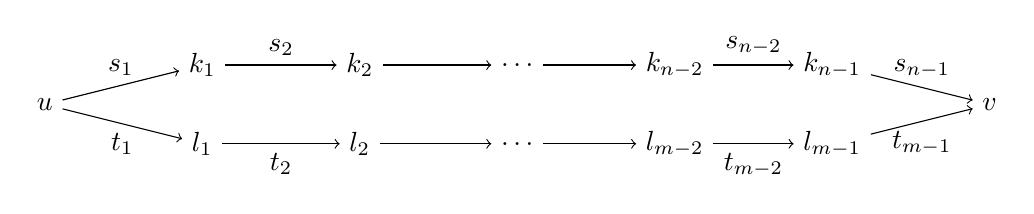
\begin{tikzpicture}
        \node (u) at (0,0) {\( u \)};
        \node (k1) at (2,0.5) {\( k_1 \)};
        \node (k2) at (4,0.5) {\( k_2 \)};
        \node (ketc) at (6,0.5) {\( \dots \)};
        \node (knm2) at (8,0.5) {\( k_{n-2} \)};
        \node (knm1) at (10,0.5) {\( k_{n-1} \)};
        \node (v) at (12,0) {\( v \)};
        \node (l1) at (2,-0.5) {\( l_1 \)};
        \node (l2) at (4,-0.5) {\( l_2 \)};
        \node (letc) at (6,-0.5) {\( \dots \)};
        \node (lnm2) at (8,-0.5) {\( l_{m-2} \)};
        \node (lnm1) at (10,-0.5) {\( l_{m-1} \)};
        \draw[->] (u) -- (k1) node [midway,above] {\( s_1 \)};
        \draw[->] (k1) -- (k2) node [midway,above] {\( s_2 \)};
        \draw[->] (k2) -- (ketc);
        \draw[->] (ketc) -- (knm2); 
        \draw[->] (knm2) -- (knm1) node[midway,above] {\( s_{n-2} \)}; 
        \draw[->] (knm1) -- (v) node[midway,above] {\( s_{n-1} \)}; 
        \draw[->] (u) -- (l1) node[midway,below] {\( t_1 \)};
        \draw[->] (l1) -- (l2) node[midway,below] {\( t_2 \)};
        \draw[->] (l2) -- (letc);
        \draw[->] (letc) -- (lnm2); 
        \draw[->] (lnm2) -- (lnm1) node[midway,below] {\( t_{m-2} \)}; 
        \draw[->] (lnm1) -- (v) node[midway,below] {\( t_{m-1} \)}; 
        \end{tikzpicture}
    }
    \end{center}
    \noindent
    the equality \( h(s_1) \star h(s_2) \star \dots  \star h(s_{n-1}) = h(t_1) \star h(t_2) \star \dots  \star h(t_{m-1}) \) holds.
\end{definition}

\begin{definition}[Pushout \cite{barr1990category}]
    \label{def:cat:po}
    \ \newline
\noindent
\begin{minipage}{0.7\textwidth}  
    A \textbf{pushout} of a span \( B \overset{\alpha}{\leftarrow} A \overset{\beta}{\rightarrow} C \), as shown on the right, is defined as a cospan \( B \overset{\beta'}{\rightarrow} D \overset{\alpha'}{\leftarrow} C \) such that \( \alpha \star \beta' = \beta \star \alpha' \), and for every cospan \( B \overset{\gamma'}{\rightarrow} E \overset{\gamma}{\leftarrow} C \), if \( \alpha \star \gamma' = \beta \star \gamma \) holds, then there exists a unique morphism \(\delta : D \to E\) such that \( \gamma' = \beta' \star \delta \) and \( \gamma = \alpha' \star \delta \).
\end{minipage}
\hfill
\begin{minipage}{0.299\textwidth}
    \hfill
\resizebox{0.9\textwidth}{!}{
           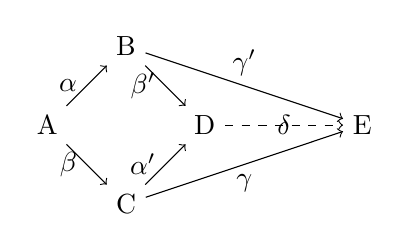
\begin{tikzpicture}
                \node (i) at (0,0) {A};
                \node (r) at (1,1) {B};
                \node (c) at (1,-1) {C};
                \node (h) at (2,0) {D};
                % \node () at (1,-1) {\( \Delta \)};
                \draw[->]  (i) -- (r) node [midway,left] {$ \alpha $};
                \draw[->] (c) -- (h) node [midway,left] {$ \alpha' $};
                \draw[->] (r) -- (h) node[midway, left] {$ \beta' $};
                \draw[->] (i) -- (c) node[midway, left] {$ \beta $};
                \node (d') at (4,0) {E};
                \draw[->] (c) -- (d') node [midway,below]{$ \gamma $};
                \draw[->] (r) -- (d') node [midway,above]{$ \gamma' $};
                \draw[->,dashed] (h) -- (d') node [midway]{$ \delta $};
            \end{tikzpicture}
}
\end{minipage}
The diagram involving \( (\alpha, \beta, \alpha', \beta') \) is called the \textbf{pushout square}, with \(D\) as the \textbf{pushout object}. The existence of a unique morphism is known as the universal mapping property of the pushout.
\end{definition} 
\begin{example}
    \label{ex:cat:po}
    Consider the square in \textbf{Graph} illustrated below.
    A pushout of the span \( B \overset{\alpha}{\leftarrowtail} A \overset{\beta}{\rightarrowtail} C \) is the cospan \( C \overset{\alpha'}{ 
    \rightarrowtail} D \overset{\beta'}{\leftarrowtail} B \), where pushout object \( D \) is the graph union of $B$ and $C$ and the morphisms \( \alpha' \) and \( \beta' \) are inclusion functions. 

    \begin{center} 
        \resizebox{0.45\textwidth}{!}{
        \begin{tikzpicture} 
            \graphbox{\( B \)}{40mm}{20mm}{34mm}{12mm}{2mm}{2mm}{
                \coordinate (o) at (0mm,-8mm); 
                \node[draw,circle] (l1) at ($(o)+(-10mm,0mm)$) {1};
                \node[draw,circle] (l2) at ($(l1)+(2,0)$) {2};
                \node[draw,circle,red] (l3) at ($(l1) + (1,0)$) {3};
                \draw[->,red] (l1) -- (l3) node[midway,above] {$a$};
                \draw[->,red] (l3) -- (l2) node[midway,above] {$a$};
            } 
    
            \graphbox{\( A \)}{0mm}{0mm}{34mm}{12mm}{2mm}{2mm}{
                \coordinate (o) at (0mm,-8mm); 
                \node[draw,circle] (l1) at ($(o)+(-10mm,0mm)$) {1};
                \node[draw,circle] (l2) at ($(l1)+(2,0)$) {2};
            }  
            \graphbox{\( D \)}{90mm}{5mm}{34mm}{22mm}{2mm}{-3mm}{
                \coordinate (o) at (0mm,-3mm); 
                \node[draw,circle] (l1) at ($(o)+(-10mm,0mm)$) {1};
                \node[draw,circle] (l2) at ($(l1)+(2,0)$) {2};
                \node[draw,circle,red] (l3) at ($(l1) + (1,0)$) {3};
                \node[draw,circle,blue] (l4) at ($(l2) + (0,-1)$) {6};
                \draw[->,red] (l1) -- (l3) node[midway,above] {$a$};
                \draw[->,red] (l3) -- (l2) node[midway,above] {$a$};
                \draw[->,blue] (l2) -- (l4) node[midway,right] {$a$};
                \node[draw,circle,blue] (l6) at ($(l1) + (0,-1)$) {7};
                \draw[<-,blue] (l1) -- (l6) node[midway,left] {$a$};
                \draw[->,blue] (l2) edge[out=-135,in=-45]node[midway,below] {$a$} (l1) ;
            }    
     
            \graphbox{\( C  \)}{40mm}{-20mm}{34mm}{22mm}{2mm}{-3mm}{
                \coordinate (o) at (0mm,-3mm); 
                \node[draw,circle] (l1) at ($(o)+(-10mm,0mm)$) {1};
                \node[draw,circle] (l2) at ($(l1)+(2,0)$) {2};
                \node[draw,circle,blue] (l4) at ($(l2) + (0,-1)$) {6};
                \draw[->,blue] (l2) -- (l4) node[midway,right] {$a$};
                \draw[->,blue] (l2) edge[out=-135,in=-45]node[midway,below] {$a$} (l1) ;
                \node[ draw,circle,blue] (l6) at ($(l1) + (0,-1)$) {7};
                \draw[<-,blue] (l1) -- (l6) node[midway,left] {$a$};
            }      
            % K to L
            \draw[>->] (17mm,5mm) -- node[above] {$\alpha$} (37mm,15mm);
            % C to G
            \draw[>->] (76mm,-28mm)-- node[below] {$\alpha'$} (104mm,-20mm) ;
            % K to C
            \draw[>->] (17mm,-17mm) -- node[below] {$\beta$} (37mm,-28mm);
            % L to G
            \draw[>->] (76mm,16mm) -- node[above] {$\beta'$} (104mm,7mm);
            \node () at (57mm,-6mm) {$PO$};
        \end{tikzpicture}
        }
    \end{center}
\end{example}
\begin{definition}[Pullback \cite{pierce1991basic}]
    \label{def:cat:pb}
    \ \newline
\noindent
\begin{minipage}{0.7\textwidth}  
   A \textbf{pullback} of a cospan \(B \overset{\beta'}{\rightarrow} D \overset{\alpha'}{\leftarrow} C \), as shown on the right, is defined as a span \( B \overset{\alpha}{\leftarrow} A \overset{\beta}{\rightarrow} C \) such that \( \alpha \star \beta' = \beta \star \alpha' \), and for every span \( B \overset{\gamma'}{\leftarrow} E \overset{\gamma}{\rightarrow} C \) if \(\gamma' \star \beta' = \gamma \star \alpha'\) holds, then there exists a unique morphism \(\delta: E \to A\) such that $\gamma' = \delta \star \alpha$ and $\gamma = \delta \star \beta$. 
\end{minipage}
\hfill
\begin{minipage}{0.299\textwidth}
    \hfill
\resizebox{0.9\textwidth}{!}{
            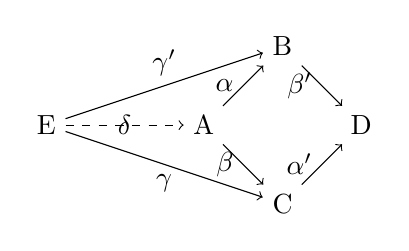
\begin{tikzpicture}
                \node (i) at (0,0) {A};
                \node (r) at (1,1) {B};
                \node (c) at (1,-1) {C};
                \node (h) at (2,0) {D};
                % \node () at (1,-1) {\( \Delta \)};
                \draw[->]  (i) -- (r) node [midway,left] {$\alpha$};
                \draw[->] (c) -- (h) node [midway,left] {$\alpha'$};
                \draw[->] (r) -- (h) node[midway, left] {$\beta'$};
                \draw[->] (i) -- (c) node[midway, left] {$\beta$};
                \node (d') at (-2,0) {E};
                \draw[<-] (c) -- (d') node [midway,below]{$\gamma$};
                \draw[<-] (r) -- (d') node [midway,above]{$\gamma'$};
                \draw[->, dashed] (d') -- (i) node [midway]{$\delta$};
            \end{tikzpicture}
}
\end{minipage}
The diagram involving \( (\alpha, \beta, \alpha', \beta') \) is called the \textbf{pullback square}, with \(A\) as the \textbf{pullback object}. The existence of a unique morphism is known as the universal mapping property of the pullback.
\end{definition} 
 
\begin{definition}
    \label{def:cat:pb}
    Consider the square in \autoref{ex:cat:po}. A pullback of the cospan \( C \overset{\alpha'}{\rightarrowtail} D \overset{\beta'}{\leftarrowtail} B \) is the span \( B \overset{\alpha}{\leftarrowtail} A \overset{\beta}{\rightarrowtail} C \), where pullback object \( A \) is the graph intersection of $B$ and $C$ and the morphisms \( \alpha \) and \( \beta \) are inclusion functions.
\end{definition}
\begin{notation}
    When the context makes it clear, a morphism \( h : A \to B \) will be denoted by \( h_{AB} \), and diagrams will be referred to by their nodes, as is standard in geometry. For example, the diagram involving morphisms \( ( \alpha, \beta, \alpha', \beta' ) \) in \autoref{def:cat:po} will be denoted by \( ACDB \) or \( ABDC \).
\end{notation}   

\section{Graph Rewriting Systems (GRS)} 

\subsection{DPO GRS}
\begin{definition}[Rewriting rule, Match~\cite{ehrig1997algebraic}]
    \label{def:grs:dpo_rule}
  A \textbf{DPO rewriting rule} $\rho$ is a span \( L \overset{l}{\leftarrow} K \overset{r}{\rightarrow} R \), where \( K \) is the \textbf{interface}, \( L \) is the \textbf{left-hand-side graph}, denoted \( \operatorname{lhs}(\rho) \), and \( R \) is the \textbf{right-hand-side graph}, denoted \( \operatorname{rhs}(\rho) \). The rule is \textbf{left-monic} if the morphism \( l \) is monic, \textbf{right-monic} if the morphism \( r \) is monic, \textbf{monic} if it is left- and right-monic \todo{Do you consider rules where this is not the case?}  
  A \textbf{match} of the rule in an graph \( G \) is a morphism \( m: L \mathop{\rightarrow} G \).   
  \end{definition}

  \begin{example}
    \label{ex:grsaa}
    The injective DPO rule from \cite[Example 6]{bruggink2014termination} will be used as a running example throughout this paper to illustrate the concepts disccussed.
    \begin{center} 
        \resizebox{0.7\textwidth}{!}{
        \begin{tikzpicture}
            \graphbox{$L$}{0mm}{0mm}{34mm}{15mm}{2mm}{-5mm}{
                \coordinate (o) at (0mm,-3mm); 
                \node[draw,circle] (l1) at ($(o)+(-10mm,0mm)$) {1};
                \node[draw,circle] (l2) at ($(l1)+(2,0)$) {2};
                \node[draw,circle] (l3) at ($(l1)+(1,0)$) {3};
                \draw[->] (l1) -- (l3) node[midway,above] {$a$};
                \draw[->] (l3) -- (l2) node[midway,above] {$a$};
            }     
            \graphbox{$K$}{40mm}{0mm}{24mm}{15mm}{2mm}{-5mm}{
                \coordinate (o) at (5mm,-3mm); 
                \node[draw,circle] (l1) at ($(o)+(-10mm,0mm)$) {1};
                \node[draw,circle] (l2) at ($(l1)+(1,0)$) {2};
                % \node[draw,circle] (l3) at ($(l1)+(1,0)$) {$\ $};
                % \draw[->] (l1) -- (l3) node[midway,above] {$a$};
                % \draw[->] (l3) -- (l2) node[midway,above] {$a$};
            }    
            \graphbox{$R$}{70mm}{0mm}{45mm}{15mm}{2mm}{-5mm}{
                \coordinate (o) at (-5mm,-3mm); 
                \node[draw,circle] (l1) at ($(o)+(-10mm,0mm)$) {1};
                \node[draw,circle] (l2) at ($(l1)+(3,0)$) {2};
                \node[draw,circle] (l3) at ($(l1)+(1,0)$) {4};
                \node[draw,circle] (l4) at ($(l1)+(2,0)$) {5};
                \draw[->] (l1) -- (l3) node[midway,above] {$a$};
                \draw[->] (l3) -- (l4) node[midway,above] {$b$};
                \draw[->] (l4) -- (l2) node[midway,above] {$a$};
            }    
            \node () at (37mm,-8mm) {$\leftarrowtail$};
            \node () at (67mm,-8mm) {$\rightarrowtail$};
            % \draw[>->] (51mm,2mm) -- (52mm,3mm);
        \end{tikzpicture}
        }
    \end{center}
  \end{example}
  
  \begin{definition}[Witness, Rewriting step \cite{endrullis2024generalized}]
    \label{def:rewriting_step}
      \ \newline
      \noindent
      \begin{minipage}{0.72\textwidth}
        A DPO diagram $\delta$ is a diagram as shown on the right.
        This diagram $\delta$ is a \textbf{witness} for the \textbf{rewriting step} from \( G \) to \( H \) using the rule \( \rho \) and match \( m \), denoted \( G \mathop{\Rightarrow}_\rho^m H \) or \( G \mathop{\Rightarrow}_\rho^\delta H \). We denote $\operatorname{left}(\delta)$ and $\operatorname{right}(\delta)$ the pushout squares $KLGC$ and $KRHC$, respectively.
      \end{minipage}
      \hfill
      \begin{minipage}{0.28\textwidth}
            % \begin{center}
            \hfill
            \resizebox{\textwidth}{!}{
            \begin{tikzpicture}
              % [node distance=11mm]
              \node (I) {$K$};
              \node (L) [left of=I] {$L$};
              \node (R) [right of=I] {$R$};
              \node (G) [below of=L] {$G$};
              \node (C) [below of=I] {$C$};
              \node (H) [below of=R] {$H$};
              \draw [->] (I) to  node [midway,above] {$l$} (L);
              \draw [->] (I) to  node [midway,above] {$r$} (R);
              \draw [->] (L) to node [midway,left] {$m$} (G);
              \draw [->] (I) to (C);
              \draw [->] (R) to node [midway,right] {$m'$} (H);
              \draw [->] (C) to node [midway,below] {$l'$} (G);
              \draw [->] (C) to node [midway,below] {$r'$} (H);
              \node [at=($(I)!.5!(G)$)] {\normalfont PO};
              \node [at=($(I)!.5!(H)$)] {\normalfont PO};
            \end{tikzpicture}
          % \end{center}
          }
          \end{minipage}
    \end{definition}

    \begin{example}
        \label{ex:rewriting_step_grs_aa}
        The DPO diagram below defines a rewriting step using the rule from Example~\ref{ex:grsaa}.
        \begin{center} 
            \resizebox{0.7\textwidth}{!}{
            \begin{tikzpicture}
                \graphbox{\( L \)}{0mm}{-3mm}{34mm}{12mm}{2mm}{2mm}{
                    \coordinate (o) at (0mm,-8mm); 
                    \node[draw,circle] (l1) at ($(o)+(-10mm,0mm)$) {1};
                    \node[draw,circle] (l2) at ($(l1)+(2,0)$) {2};
                    \node[draw,circle] (l3) at ($(l1)+(1,0)$) {3};
                    \draw[->] (l1) -- (l3) node[midway,above] {$a$};
                    \draw[->] (l3) -- (l2) node[midway,above] {$a$};
                } 
        
                \graphbox{\( K \)}{40mm}{-3mm}{34mm}{12mm}{2mm}{2mm}{
                    \coordinate (o) at (0mm,-8mm); 
                    \node[draw,circle] (l1) at ($(o)+(-10mm,0mm)$) {1};
                    \node[draw,circle] (l2) at ($(l1)+(2,0)$) {2};
                }  
        
                \graphbox{\( R \)}{80mm}{-3mm}{45mm}{12mm}{2mm}{2mm}{
                    \coordinate (o) at (-5mm,-8mm); 
                    \node[draw,circle] (l1) at ($(o)+(-10mm,0mm)$) {1};
                    \node[draw,circle] (l2) at ($(l1)+(3,0)$) {2};
                    \node[draw,circle] (l3) at ($(l1)+(1,0)$) {4};
                    \node[draw,circle] (l4) at ($(l1)+(2,0)$) {5};
                    \draw[->] (l1) -- (l3) node[midway,above] {$a$};
                    \draw[->] (l3) -- (l4) node[midway,above] {$b$};
                    \draw[->] (l4) -- (l2) node[midway,above] {$a$};
                }    
        
                \graphbox{\( G \)}{0mm}{-22mm}{34mm}{22mm}{2mm}{-3mm}{
                    \coordinate (o) at (0mm,-3mm); 
                    \node[draw,circle] (l1) at ($(o)+(-10mm,0mm)$) {1};
                    \node[draw,circle] (l2) at ($(l1)+(2,0)$) {2};
                    \node[draw,circle] (l3) at ($(l1)+(1,0)$) {3};
                    \node[draw,circle] (l4) at ($(l2)+(0,-1)$) {6};
                    \draw[->] (l1) -- (l3) node[midway,above] {$a$};
                    \draw[->] (l3) -- (l2) node[midway,above] {$a$};
                    \draw[->] (l2) -- (l4) node[midway,right] {$a$};
                    \node[draw,circle] (l6) at ($(l1)+(0,-1)$) {7};
                    \draw[<-] (l1) -- (l6) node[midway,left] {$a$};
                    \draw[->] (l2) edge[out=-135,in=-45]node[midway,below] {$a$} (l1) ;
                }    
        
                \graphbox{\( C  \)}{40mm}{-22mm}{34mm}{22mm}{2mm}{-3mm}{
                    \coordinate (o) at (0mm,-3mm); 
                    \node[draw,circle] (l1) at ($(o)+(-10mm,0mm)$) {1};
                    \node[draw,circle] (l2) at ($(l1)+(2,0)$) {2};
                    \node[draw,circle] (l4) at ($(l2)+(0,-1)$) {6};
                    \draw[->] (l2) -- (l4) node[midway,right] {$a$};
                    \draw[->] (l2) edge[out=-135,in=-45]node[midway,below] {$a$} (l1) ;
                    \node[ draw,circle] (l6) at ($(l1)+(0,-1)$) {7};
                    \draw[<-] (l1) -- (l6) node[midway,left] {$a$};
                }    
        
                \graphbox{\( H \)}{80mm}{-22mm}{45mm}{22mm}{2mm}{-3mm}{
                    \coordinate (o) at (-5mm,-3mm); 
                    \node[draw,circle] (l1) at ($(o)+(-10mm,0mm)$) {1};
                    \node[draw,circle] (l2) at ($(l1)+(3,0)$) {2};
                    \node[draw,circle] (l3) at ($(l1)+(1,0)$) {4};
                    \node[draw,circle] (l4) at ($(l1)+(2,0)$) {5};
                    \node[ draw,circle] (l5) at ($(l2)+(0,-1)$) {6};
                    \node[ draw,circle] (l6) at ($(l1)+(0,-1)$) {7};
                    \draw[<-] (l1) -- (l6) node[midway,left] {$a$};
                    \draw[->] (l1) -- (l3) node[midway,above] {$a$};
                    \draw[->] (l3) -- (l4) node[midway,above] {$b$};
                    \draw[->] (l4) -- (l2) node[midway,above] {$a$};
                    \draw[->] (l2) -- (l5) node[midway,right] {$a$};
                    \draw[->] (l2) edge[out=-135,in=-45]node[midway,below] {$a$} (l1) ;
                }    
        
                \node () at (37mm,-8mm) {\( \leftarrowtail \)}; % K -> L
                \node () at (77mm,-8mm) {\( \rightarrowtail \)}; % K -> R
                \node () at (15mm,-18mm) {\( m\ \downarrowtail \)};
                \node () at (37mm,-33mm) {\( \leftarrowtail \)};
                \node () at (58mm,-18mm) {\( \downarrowtail \)};
                \node () at (102mm,-18mm) {\( \downarrowtail \)};
                \node () at (77mm,-33mm) {\( \rightarrowtail \)}; % C -> H
            \end{tikzpicture}
            }
        \end{center}
      \end{example}

\begin{definition}[Rewriting framework \cite{endrullis2024generalized}]
    A \textbf{DPO rewriting framework} $\mathfrak{F}$ is a mapping of DPO rewriting rules to classes of DPO diagrams such that, for every rule $\rho$, $\mathfrak{F}(\rho)$ is a class of DPO diagrams with top-span $\rho$.
  \end{definition}

\begin{definition}[Rewriting relation]
  The \textbf{rewriting relation $\mathop{\Rightarrow}_{\mathfrak{dpo},\mathfrak{F},\rho}$ induced by a rule $\rho$ in $\mathfrak{F}$} is defined as follows: $G \mathop{\Rightarrow}_{\mathfrak{dpo},\mathfrak{F},\rho} H$ iff $G \mathop{\Rightarrow}_\rho^\delta H$ for some $\delta \mathop{\in} \mathfrak{F}(\rho)$. 
    % for some $\delta \mathop{\in} \mathfrak{F}(\rho)$
     The \textbf{DPO rewriting relation $\mathop{\Rightarrow}_{\mathcal{R},\mathfrak{F}}$ induced by a set $\mathcal{R}$ of DPO rewriting rules in $\mathfrak{F}$} is given by: $G \mathop{\Rightarrow}_{\mathfrak{dpo}, \mathfrak{F},\mathcal{R}} H$ iff $G \mathop{\Rightarrow}_{\mathfrak{dpo},\mathfrak{F}, \rho} H$ for some $\rho \mathop{\in} \mathcal{R}$. When $\mathfrak{F}$ is clear from the context, we 
    suppress $\mathfrak{F}$ and 
    write $\mathop{\Rightarrow}_{\mathfrak{dpo},\rho}$ and $\mathop{\Rightarrow}_{\mathfrak{dpo},\mathcal{R}}$.
\end{definition}
% % \begin{definition}[Rewriting relation]
    % The \textbf{DPO rewriting relation $\Rightarrow_{\rho,\mathfrak{F},A}$ induced by a DPO rewriting rule $\rho$ in $\mathfrak{F}$ with the set $A$ of negative application condition over $\rho$} is defined as follows: $G \Rightarrow_{\rho,\mathfrak{F},A} H$ iff $G \Rightarrow_\rho^m H$ for some match $m$ such that there does not exist a negative application condition $(f:X \rightarrowtail F) \in A$ such that $f \star g = m$ for some monomorphism $g: F \rightarrowtail G$.
    % Let $\mathcal{R}$ be a set of DPO rewriting rules, $\operatorname{NAC}$ a function which associates a set of negative application conditions to each rule in $\mathcal{R}$ and $\mathfrak{F}$ a DPO rewriting framework.
    % The \textbf{DPO rewriting relation $\Rightarrow_{\mathcal{R},\mathfrak{F},\operatorname{NAC}}$ induced by $\mathcal{R}$ in $\mathfrak{F}$ with $\operatorname{NAC}$} is given by: $G \Rightarrow_{\mathcal{R}, \mathfrak{F},\operatorname{NAC}} H$ iff $G \Rightarrow_{\rho, \mathfrak{F},\operatorname{NAC}(\rho)} H$ for some $\rho \in \mathcal{R}$. 
    % When $\mathfrak{F}$ is clear from the context, we 
    % suppress $\mathfrak{F}$ and 
    % write $\Rightarrow_{\rho,A}$ and $\Rightarrow_{\mathcal{R},\operatorname{NAC}}$.
    The \textbf{DPO rewriting relation $\Rightarrow_{\rho,\mathfrak{F}}$ induced by a DPO rewriting rule $\rho$ in $\mathfrak{F}$} is defined as follows: $G \Rightarrow_{\rho,\mathfrak{F}} H$ iff $G \Rightarrow_\rho^\delta H$ for some $\delta \in \mathfrak{F}(\rho)$. 
    % for some $\delta \in \mathfrak{F}(\rho)$
    The \textbf{DPO rewriting relation $\Rightarrow_{\mathcal{R},\mathfrak{F}}$ induced by a set $\mathcal{R}$ of DPO rewriting rules in $\mathfrak{F}$} is given by: $G \Rightarrow_{\mathcal{R},\mathfrak{F}} H$ iff $G \Rightarrow_{\rho,\mathfrak{F}} H$ for some $\rho \in \mathcal{R}$. When $\mathfrak{F}$ is clear from the context, we 
    suppress $\mathfrak{F}$ and 
    write $\Rightarrow_{\rho}$ and $\Rightarrow_{\mathcal{R}}$.
\end{definition}

 
% Throughout this chapter, unless otherwise specified,
% % \(\mathfrak{F}\) denotes the DPO rewriting framework which associates each rule with the class of all DPO diagrams with the rule as the top span, and 
% \(\mathfrak{M}\) denotes the DPO rewriting framework which associates each rule with the class of all DPO diagrams with monic matches and the rule as the top span. 
\color{red}    


dpo
dpo limitations ;
les autres differences

\begin{proposition}[to do]
    inclusion : dpo $>$ spo $>$ ...
\end{proposition}

\begin{itemize}
    \item we are only able to delete nodes if they do not leave any edges “dangling” (called the gluing condition),This can be considered a pleasant safety feature, but also a limitation. However, since GLS never delete or duplicate nodes, DPO GRS is a well studied approach with advanced termination method.
    \item the most dominant graph rewriting method, called the Double Pushout (DPO) approach, combines the pushout complement approach (with the injectivity requirement on $\rho$) with the ToyPO approach. In doing so, it enables the specification of rewrite steps with deletion, identification and addition features, for matches m that satisfy the gluing condition.
    \item Alternatives to the DPO approach avoid the construction of pushout complements. For instance, the Single Pushout (SPO) approach [17] relies on a single pushout construction, but uses partial graph homomorphisms instead of total morphisms, in order to specify deletion. In this approach, the gluing condition no longer needs to be checked either: all edges incident to a removed vertex are simply deleted.
    \item As another example, the Sesqui-Pushout (corradini2006sesqui) approach [8] replaces the first PO square of DPO by what is called a final pullback complement square. This square allows duplication with deterministic behavior, and like SPO, deletes any edges that would be left dangling.
    \item !!! implicite deletion of nodes or edges is a problem when we want to prove the termination 
    \item[handbook] 
        As shown for example in [2], in category Graph, the pushout complement object of two morphisms <b,g> exsits iff the gluing condition is satisfied; moreover, it is unique if b is injective.
        \begin{proposition}[Existence of Pushout Complements]
            Let $b : A \mathop{\to} B$ and $g : B \mathop{\to} D$ be two morphisms in $\mathbf{Graph}$. Then there exists a pushout complement $\langle C, c : A \mathop{\to} C, f : C \mathop{\to} D \rangle$ of $\langle b, g \rangle$ if and only if the following conditions are satisfied:
            
            \begin{itemize}
                \item \textbf{[Dangling condition]} No edge $e \mathop{\in} D_E - g_E(B_E)$ is incident to any node in $g_V(B_V - b_V(A_V))$.
                \item \textbf{[Identification condition]} There is no $x, y \mathop{\in} B_V \mathop{\cup} B_E$ such that $x \mathop{\neq} y$, $g(x) \mathop{=} g(y)$ and $y \notin b(A_V \mathop{\cup} A_E)$.
            \end{itemize}
            
            In this case, we say that $\langle b, g \rangle$ satisfies the \textit{gluing condition} (or $g$ satisfies the gluing condition with respect to $b$). If moreover morphism $b$ is injective, then the pushout complement is unique up to isomorphism, i.e., if $\langle C, c, f \rangle$ and $\langle C', c', f' \rangle$ are two pushout complements of $\langle b, g \rangle$, then there is an isomorphism $\varphi : C \mathop{\to} C'$ such that $\varphi \circ c \mathop{=} c'$ and $f' \circ \varphi \mathop{=} f$.
            \end{proposition}
        
    \item[adhesive categories] In D-p rewriting, a rewrite rule is given as a span 
    \begin{tikzcd}
        L & K \arrow[l] \arrow[r] & R
    \end{tikzcd}. 
    Roughly, The intuition is that \( L \) forms the left-hand side of the rewrite rule, \( R \) forms the right-hand side and \( K \), common to both \( L \) and \( R \), is the sub-structure to be unchanged as the rule is applied. To apply the rule to a structure \( C \), one first needs to find a match \( L \mathop{\to} C \) of \( L \) within \( C \). The rule is then applied by constructing the missing parts (\( E, D \) and arrows) of the following diagram
    \begin{figure}[H]
        \begin{tikzcd}
            L \arrow[d]&  K \arrow[d] \arrow[l] \arrow[r] & R  \arrow[d]\\
            C  & E \arrow[l]  \arrow[r] & D
        \end{tikzcd} 
    \end{figure}
    in a way which ensures that the two squares are pushout diagrams. Once such a diagram is constructed we may deduce that \( C \mathop{\Rightarrow} D \), that is, \( C \) rewrites to \( D \).
    
\end{itemize}



\begin{definition}[DPO Graph Rewriting System \cite{endrullis2024generalized}]
    A \textbf{DPO Graph Rewriting System} is a DPO rewriting system on $\mathbf{Graph}$.  
\end{definition}

When a direct graph transformation with a production p and a match m is performed, all the vertices and edges which are matched by$ L \mathop{\setminus} K$ are removed from G. The removed part is not a graph, in general, but the remaining structure $D := (G \mathop{\setminus} m(L)) \mathop{\cup}  m(K)$ still has to be a graph. This means that the match $m$ has to satisfy a suitable gluing condition, which makes sure that the gluing of $L\mathop{\setminus} K$ and $D$ is equal to G. In the second step of a graph rewriting step, the graph $D$ is glued together with $R \mathop{\setminus} K$ to obtain the derived graph $H$ . For gluing newly created vertices and edges into D,the graph $m(K)$ and $r(K)$ are used: nodes and edges with the same pre-image will be unified.

Trees form a sub-category of $\mathbf{Graph}$, denoted as $\mathbf{Tree}$.
\begin{definition}[DPO Tree Rewriting System]
   A \textbf{DPO Tree Rewriting System} is a DPO rewriting system on $\mathbf{Tree}$.
\end{definition}

todo : Def functor F
\begin{proposition} 
   The functor $F: \mathbf{Tree} \mathop{\to} \mathbf{Trs}$ is isomorphic.
\end{proposition}
todo : def functor F
\begin{proposition}
   
   $F$ is a functor from the category of GLS to the category of linear DPO graph rewriting.
\end{proposition}

\begin{remark}
   a GLS is essentially a DPO GRS. Its simplicity compare with respect to DPO GRS is that, in the definition of rewriting step,it replaces the DPO diagram by "the underlying graph does not change", and deletion add addition of labeled arrows by the relabeling of unlabeled arrows. Its semantic is more intuitive but there is a price to pay compare to DPO GRS: we need to constantly renaming nodes. 
\end{remark}

\begin{remark}
  A TRS is essentially a DPO Tree rewriting system, which replace the DPO diagram in the definition of rewriting stemp by choosing the root node of lhs and rhs terms as interface (which is a very intuitive choice). A part hitorical, there is no reason to prefer TRS to DPO Tree rewriting.
\end{remark}
\color{black} 

\subsection{DPO GRS with Negative Application Condition}
\begin{definition}[Rewriting rule, Match~\cite{bottoni2010atermination}]
    \label{def:grs:dpo_nac_rule}
    A \textbf{DPO rewriting rule with a negative application condition} $\varphi$ is an ordered pair \( \left( n , \rho \right) \) where $n$ is a monomorphism and $\rho$ is an monic DPO rewriting rule
     such that $\operatorname{codom}(\operatorname{lhs}(\rho)) \mathop{=} \operatorname{dom}(n)$.
     
     A rule is denoted \( N \overset{n}{\leftarrowtail} L \overset{l}{\leftarrowtail} K \overset{r}{\rightarrowtail} R \) with $\rho \mathop{=} (L \overset{l}{\leftarrowtail} K \overset{r}{\rightarrowtail} R) $.

    A match of the rule in an object \( G \) is a monomorphism \( m: L \mathop{\rightarrow} G \) such that there is no monomorphism \( q: N \mathop{\rightarrow} G \) such that \( n \mathop{\star} q \mathop{=} m \), as illustrated below.

    A DPO diagram as shown below is a \textbf{witness} for a \textbf{rewriting step} from \( G \) to \( H \) using the rule $\varphi$ and match \( m \), denoted \( G \mathop{\Rightarrow}_\rho^m H \) or \( G \mathop{\Rightarrow}_\rho^\delta H \). 
    % We denote $\operatorname{left}(\delta)$ and $\operatorname{right}(\delta)$ the pushout squares $KLGC$ and $KRHC$, respectively.

\begin{figure}[htbp]
    \begin{tikzpicture} 
        % Define nodes
        \node (K)  {K};
        \node (L) [left=of K] {L};
        \node (R) [right=of K] {R};
        \node (N) [left=of L] {N};
        \node (G) [below=of L] {G};
        \node (D) [below=of K] {D};
        \node (H) [below=of R] {H};

        % Draw arrows
        % Top row
        \draw[>->] (L) -- node[above] {n} (N);
        \draw[>->] (K) -- node[above] {$l$} (L);
        \draw[>->] (K) -- node[above] {$r$} (R);
      
        % Vertical arrows
        \draw[>->] (L) -- node[left] {$m$} (G);
        \draw[>->] (K) --  (D);
        \draw[>->] (R) --  (H);
      
        % Bottom row
        \draw[>->] (G) --  (D);
        \draw[>->] (D) --   (H);
      
        % Bent arrow from G to N
        \draw[>->, bend right,red,dashed] (N) to node[below] {q} (G);

        \node at ($(N)!0.5!(G)$) {\textcolor{red}{$\mathop{\neq}$}};
        \node at ($(K)!0.5!(G)$) {$\mathrm{PO}$};
        \node at ($(K)!0.5!(H)$) {$\mathrm{PO}$};
      \end{tikzpicture}
      \label{fig:grs:dpo_nac_rule}
\end{figure}
\end{definition}
\begin{example}
  The following diagram illustrates a DPO rewriting rule with a negative application condition:
  \begin{center} 
    \resizebox{0.7\textwidth}{!}{
    \begin{tikzpicture}
      \graphbox{$N$}{-40mm}{0mm}{34mm}{20mm}{2mm}{-5mm}{
        \coordinate (o) at (0mm,-3mm); 
        \node[draw,circle] (l1) at ($(o)+(-10mm,0mm)$) {1};
        \node[draw,circle] (l2) at ($(l1)+(2,0)$) {2};
        \node[draw,circle] (l3) at ($(l1)+(1,0)$) {3};
        \draw[->] (l1) -- (l3) node[midway,above] {$a$};
        \draw[->] (l3) -- (l2) node[midway,above] {$a$};
        \draw[->] (l2) edge[out=-135,in=-45]node[midway,below] {$a$} (l1) ;
    }  
        \graphbox{$L$}{0mm}{0mm}{34mm}{15mm}{2mm}{-5mm}{
            \coordinate (o) at (0mm,-3mm); 
            \node[draw,circle] (l1) at ($(o)+(-10mm,0mm)$) {1};
            \node[draw,circle] (l2) at ($(l1)+(2,0)$) {2};
            \node[draw,circle] (l3) at ($(l1)+(1,0)$) {3};
            \draw[->] (l1) -- (l3) node[midway,above] {$a$};
            \draw[->] (l3) -- (l2) node[midway,above] {$a$};
        }     
        \graphbox{$K$}{40mm}{0mm}{24mm}{15mm}{2mm}{-5mm}{
            \coordinate (o) at (5mm,-3mm); 
            \node[draw,circle] (l1) at ($(o)+(-10mm,0mm)$) {1};
            \node[draw,circle] (l2) at ($(l1)+(1,0)$) {2};
            % \node[draw,circle] (l3) at ($(l1)+(1,0)$) {$\ $};
            % \draw[->] (l1) -- (l3) node[midway,above] {$a$};
            % \draw[->] (l3) -- (l2) node[midway,above] {$a$};
        }    
        \graphbox{$R$}{70mm}{0mm}{45mm}{15mm}{2mm}{-5mm}{
            \coordinate (o) at (-5mm,-3mm); 
            \node[draw,circle] (l1) at ($(o)+(-10mm,0mm)$) {1};
            \node[draw,circle] (l2) at ($(l1)+(3,0)$) {2};
            \node[draw,circle] (l3) at ($(l1)+(1,0)$) {4};
            \node[draw,circle] (l4) at ($(l1)+(2,0)$) {5};
            \draw[->] (l1) -- (l3) node[midway,above] {$a$};
            \draw[->] (l3) -- (l4) node[midway,above] {$b$};
            \draw[->] (l4) -- (l2) node[midway,above] {$a$};
        }    
        \node () at (-3mm,-8mm) {$\leftarrowtail$};
        \node () at (37mm,-8mm) {$\leftarrowtail$};
        \node () at (67mm,-8mm) {$\rightarrowtail$};
        % \draw[>->] (51mm,2mm) -- (52mm,3mm);
    \end{tikzpicture}
    }
\end{center}
  The rewriting step in Example~\ref{ex:rewriting_step_grs_aa} is not possible with this rule in DPO rewriting with negative application conditions, because there exists a monomorphism \( q: N \mathop{\rightarrow} G \) such that \( n \mathop{\star} q \mathop{=} m \) as shown in the diagram below.
  \begin{center} 
    \resizebox{0.7\textwidth}{!}{
    \begin{tikzpicture}
      \graphbox{$N$}{-40mm}{0mm}{34mm}{20mm}{2mm}{-5mm}{
        \coordinate (o) at (0mm,-3mm); 
        \node[draw,circle] (l1) at ($(o)+(-10mm,0mm)$) {1};
        \node[draw,circle] (l2) at ($(l1)+(2,0)$) {2};
        \node[draw,circle] (l3) at ($(l1)+(1,0)$) {3};
        \draw[->] (l1) -- (l3) node[midway,above] {$a$};
        \draw[->] (l3) -- (l2) node[midway,above] {$a$};
        \draw[->] (l2) edge[out=-135,in=-45]node[midway,below] {$a$} (l1) ;
    }  
        \graphbox{\( L \)}{0mm}{-3mm}{34mm}{12mm}{2mm}{2mm}{
            \coordinate (o) at (0mm,-8mm); 
            \node[draw,circle] (l1) at ($(o)+(-10mm,0mm)$) {1};
            \node[draw,circle] (l2) at ($(l1)+(2,0)$) {2};
            \node[draw,circle] (l3) at ($(l1)+(1,0)$) {3};
            \draw[->] (l1) -- (l3) node[midway,above] {$a$};
            \draw[->] (l3) -- (l2) node[midway,above] {$a$};
        } 

        \graphbox{\( K \)}{40mm}{-3mm}{34mm}{12mm}{2mm}{2mm}{
            \coordinate (o) at (0mm,-8mm); 
            \node[draw,circle] (l1) at ($(o)+(-10mm,0mm)$) {1};
            \node[draw,circle] (l2) at ($(l1)+(2,0)$) {2};
        }  

        \graphbox{\( R \)}{80mm}{-3mm}{45mm}{12mm}{2mm}{2mm}{
            \coordinate (o) at (-5mm,-8mm); 
            \node[draw,circle] (l1) at ($(o)+(-10mm,0mm)$) {1};
            \node[draw,circle] (l2) at ($(l1)+(3,0)$) {2};
            \node[draw,circle] (l3) at ($(l1)+(1,0)$) {4};
            \node[draw,circle] (l4) at ($(l1)+(2,0)$) {5};
            \draw[->] (l1) -- (l3) node[midway,above] {$a$};
            \draw[->] (l3) -- (l4) node[midway,above] {$b$};
            \draw[->] (l4) -- (l2) node[midway,above] {$a$};
        }    

        \graphbox{\( G \)}{0mm}{-22mm}{34mm}{22mm}{2mm}{-3mm}{
            \coordinate (o) at (0mm,-3mm); 
            \node[draw,circle] (l1) at ($(o)+(-10mm,0mm)$) {1};
            \node[draw,circle] (l2) at ($(l1)+(2,0)$) {2};
            \node[draw,circle] (l3) at ($(l1)+(1,0)$) {3};
            \node[draw,circle] (l4) at ($(l2)+(0,-1)$) {6};
            \draw[->] (l1) -- (l3) node[midway,above] {$a$};
            \draw[->] (l3) -- (l2) node[midway,above] {$a$};
            \draw[->] (l2) -- (l4) node[midway,right] {$a$};
            \node[draw,circle] (l6) at ($(l1)+(0,-1)$) {7};
            \draw[<-] (l1) -- (l6) node[midway,left] {$a$};
            \draw[->] (l2) edge[out=-135,in=-45]node[midway,below] {$a$} (l1) ;
        }    

        \graphbox{\( C  \)}{40mm}{-22mm}{34mm}{22mm}{2mm}{-3mm}{
            \coordinate (o) at (0mm,-3mm); 
            \node[draw,circle] (l1) at ($(o)+(-10mm,0mm)$) {1};
            \node[draw,circle] (l2) at ($(l1)+(2,0)$) {2};
            \node[draw,circle] (l4) at ($(l2)+(0,-1)$) {6};
            \draw[->] (l2) -- (l4) node[midway,right] {$a$};
            \draw[->] (l2) edge[out=-135,in=-45]node[midway,below] {$a$} (l1) ;
            \node[ draw,circle] (l6) at ($(l1)+(0,-1)$) {7};
            \draw[<-] (l1) -- (l6) node[midway,left] {$a$};
        }    

        \graphbox{\( H \)}{80mm}{-22mm}{45mm}{22mm}{2mm}{-3mm}{
            \coordinate (o) at (-5mm,-3mm); 
            \node[draw,circle] (l1) at ($(o)+(-10mm,0mm)$) {1};
            \node[draw,circle] (l2) at ($(l1)+(3,0)$) {2};
            \node[draw,circle] (l3) at ($(l1)+(1,0)$) {4};
            \node[draw,circle] (l4) at ($(l1)+(2,0)$) {5};
            \node[ draw,circle] (l5) at ($(l2)+(0,-1)$) {6};
            \node[ draw,circle] (l6) at ($(l1)+(0,-1)$) {7};
            \draw[<-] (l1) -- (l6) node[midway,left] {$a$};
            \draw[->] (l1) -- (l3) node[midway,above] {$a$};
            \draw[->] (l3) -- (l4) node[midway,above] {$b$};
            \draw[->] (l4) -- (l2) node[midway,above] {$a$};
            \draw[->] (l2) -- (l5) node[midway,right] {$a$};
            \draw[->] (l2) edge[out=-135,in=-45]node[midway,below] {$a$} (l1) ;
        }    
        \draw[>->, bend right,red] (-21mm,-22mm) to node[below] {q} (-4mm,-33mm);
        \node () at (-3mm,-8mm) {$\leftarrowtail$};
        \node () at (37mm,-8mm) {\( \leftarrowtail \)}; % K -> L
        \node () at (77mm,-8mm) {\( \rightarrowtail \)}; % K -> R
        \node () at (15mm,-18mm) {\( m\ \downarrowtail \)};
        \node () at (37mm,-33mm) {\( \leftarrowtail \)};
        \node () at (58mm,-18mm) {\( \downarrowtail \)};
        \node () at (102mm,-18mm) {\( \downarrowtail \)};
        \node () at (77mm,-33mm) {\( \rightarrowtail \)}; % C -> H
    \end{tikzpicture}
    }
\end{center}
\end{example}

\begin{definition}[Rewriting framework]
  A framework of rewriting with a negative application condition $\mathfrak{F}$ is a mapping of DPO rewriting rules with a negative condition to classes of diagrams as illustrated in Definition~\ref{def:grs:dpo_nac_rule} such that, for every rule $\varphi =(n, \rho)$, every diagram in $\mathfrak{F}(\varphi)$ has $\rho$ as the top-span of the DPO subdiagram.
\end{definition}

\begin{definition}[Rewriting relation]
  The \textbf{rewriting relation $\mathop{\Rightarrow}_{\mathfrak{dponac},\mathfrak{F},\rho}$ induced by a rule $\rho$ in $\mathfrak{F}$} is defined as follows: $G \mathop{\Rightarrow}_{\mathfrak{dponac},\mathfrak{F},\rho} H$ iff $G \mathop{\Rightarrow}_\rho^\delta H$ for some $\delta \mathop{\in} \mathfrak{F}(\rho)$. 
    % for some $\delta \mathop{\in} \mathfrak{F}(\rho)$
     The \textbf{DPO rewriting relation $\mathop{\Rightarrow}_{\mathfrak{dponac},\mathfrak{F},\mathcal{R}}$ induced by a set $\mathcal{R}$ of DPO rewriting rules in $\mathfrak{F}$} is given by: $G \mathop{\Rightarrow}_{\mathfrak{dponac}, \mathfrak{F},\mathcal{R}} H$ iff $G \mathop{\Rightarrow}_{\mathfrak{dponac},\mathfrak{F}, \rho} H$ for some $\rho \mathop{\in} \mathcal{R}$. When $\mathfrak{F}$ is clear from the context, we 
    suppress $\mathfrak{F}$ and 
    write $\mathop{\Rightarrow}_{\mathfrak{dponac},\rho}$ and $\mathop{\Rightarrow}_{\mathfrak{dponac},\mathcal{R}}$.
\end{definition}

\subsection{PBPO+ GRS}
\textcolor{red}{qq: PBPO+ can simulate term rewriting system with a termination preservation, but tree structure of the context will be lost if we use the translation proposed by endrusllis and overbeek}

\textcolor{red}{PBPO+ requires only pullbacks, and pushouts along monomorphisms}
\begin{definition}[PBPO+ Rewriting Rule~\cite{overbeek2023pbpo_JLAMP}]
  \label{def:pbpop:rule}
  A \pbpop \textbf{rewriting rule} \(\rho\) is a diagram of the form
\begin{center}

\begin{tikzpicture}[node distance=12mm, auto]

\node (L) {$L$};
\node (K) [right=of L] {$K$};
\node (R) [right=of K] {$R$};

\node (L') [below=of L] {$L'$};
\node (K') [below=of K] {$K'$};

% Arrows for the upper row
\draw[<-] (L) to node [above] {$l$} (K);
\draw[->] (K) to node [above] {$r$} (R);

% Vertical arrows 
\draw[->] (L) to node [left] {$t_L$} (L');
\draw[->] (K) to node [right] {$t_K$} (K');

% Arrows for the lower row
\draw[<-] (L') to node [below] {$l'$} (K');

% Pullback label
\node at ($(L)!0.5!(K')$) {$PB$};
\end{tikzpicture}
\end{center}

\noindent where \(L\), \(K\) and \(R\) are the input, interface and output patterns; \(L'\) is the context type of $L$, and \(t_L\) is the context typing of $L$; \(K'\) the context type of $K$, and \(t_K\) is the context typing of $K$. 
\end{definition} 
\textcolor{red}{intuition:
L is the pattern; L' restricts the shape of the context; pullback: duplication and filtering(extraction); pushout:merging and extension; strong matching: leftmost pullback square ensures that the context in $G_L$ is not mapped onto the pattern L in L'
}

The morphism \(l' : L' \mathop{\leftarrow} K'\) is used to define deletion and duplication operations on the type graph. The morphism \(r : K \mathop{\to} R\) subsequently specifies the identification and addition operations, particularly focused on \(l'^{-1}(t_L)\).
% For PBPO\(^*\) matches, it is required that \(\alpha^{-1}(\operatorname{Im} t_L) \overset{iso}{=} L\). Such a match is called a \textit{strong match}, which distinguishes $PBPO+$ from $PBPO$, and is uniquely determined by the means of an adherence morphism.
\begin{example}
    \url{https://www.youtube.com/watch?v=_gwz64o1eBQ&t=1352s} 30:20 an example of a rule which remove a single loop from a graph.
\end{example}
\begin{definition}[Match]
  A \textbf{match} of a \pbpop rewriting rule \(\rho\) in an object \(G\) is an ordered pair of morphisms \(m:L\rightarrow G, \alpha: G \mathop{\rightarrow} L'\) such that the following square is a pullback square:

  \[
  \begin{tikzcd}[row sep=large, column sep=large]
  L \arrow[r, "m"] \arrow[d, equals] & G \arrow[d, "\alpha"] \\
  L \arrow[r, "t_L"] & L'
  \arrow[phantom, from=1-1, to=2-2, "\mathrm{PB}" {pos=0.5, inner sep=1pt}]
  \end{tikzcd}
  \]
  \end{definition}

\begin{proposition}
  In any category, if diagrams
\[
\begin{tikzcd}
L \arrow[r, "m'"] \arrow[d, equals] & G \arrow[d, "m"] \\
L \arrow[r, "t_L"] & L'
\arrow[phantom, from=1-1, to=2-2, "\mathrm{PB}" description]
\end{tikzcd}
\quad \text{and} \quad
\begin{tikzcd}
L \arrow[r, "m''"] \arrow[d, equals] & G \arrow[d, "m"] \\
L \arrow[r, "t_L"] & L'
\arrow[phantom, from=1-1, to=2-2, "\mathrm{=}" description]
\end{tikzcd}
\]
hold then $m' \mathop{=} m''$.
\end{proposition}

\begin{definition}[\pbpop rewrite step~\cite{overbeek2023pbpo_JLAMP}]
  Let $\rho$ be a \pbpop rewriting rule as illustrated in Definition~\ref{def:pbpop:rule}. 

  Let $G_L$ be an object and \(m, \alpha\) a match. 
  
 A diagram as illustrated below, where \(u : K \mathop{\rightarrow} G_K\) is the unique morphism satisfying \(t_K \mathop{=} u' \circ u\), is a \textbf{witness} of a \pbpop \textbf{rewrite step} from $G_L$ to $G_R$ using rule $\rho$ and match $m$, denoted \(G_L \mathop{\Rightarrow}^m_{\text{\pbpop},\rho} G_R\).

  \begin{tikzpicture} 
    % Nodes of the diagram
      \node (L) {$L$};
      \node (GL) [right=of L] {$G_L$};
      \node (GK) [right=of GL] {$G_K$};
      \node (K) [above=of GK] {$K$};
      \node (R) [right=of K] {$R$};
      \node (GR) [below=of R] {$G_R$};

      \node (L2) [below=of L] {$L$};
      \node (L') [right=of L2] {$L'$};
      \node (K') [right=of L'] {$K'$};

      % Arrows on the top row
      \draw[->] (L) to node [above] {$m$} (GL);
      \draw[->] (K) to node [above] {$r$} (R);
      \draw[<-] (GL) to node [above] {$g_L$} (GK);
      \draw[->] (GK) to node [left] {$u'$} (K');
      \draw[<-,dashed] (GK) to node [left] {$!u$} (K);
      \draw[->] (R) to node [right] {$w$} (GR);
      \draw[->] (GK) to node [above] {$g_R$} (GR);

      % Arrows on the bottom row
      \draw[->] (L2) to node [above] {$t_L$} (L');
      \draw[<-] (L') to node [above] {$l'$} (K');

      % Vertical arrows
      \draw[->] (GL) to node [right] {$\alpha$} (L');
      \draw[=] (L) to node [left] {} (L2);

      % Curved arrow from K to GK
      \draw[->] (K) to [bend left] node [pos=0.75,right] {$t_K$} (K');

      % PB and PO labels
      \node at ($(L)!0.5!(L')$) {$PB$};
      \node at ($(GK)!0.5!(L')$) {$PB$};
      \node at ($(K)!0.5!(GR)$) {$PO$}; 
  \end{tikzpicture}
\end{definition}

\begin{definition}[Rewriting framework]
  A \pbpop \textbf{rewriting framework} $\mathfrak{F}$ is a mapping associating to each \pbpop rule $\rho$ as depicted in Definition~\ref{def:pbpop:rule} 
   the class of \pbpop witnesses of form as illustrated in Definition~\ref{def:pbpop:rule}.
\end{definition}

\begin{definition}[Rewriting relation]
  The \textbf{rewriting relation $\mathop{\Rightarrow}_{\text{\pbpop},\mathfrak{F},\rho} $ induced by a rule $\rho$ in $\mathfrak{F}$} is defined as follows: $G_L \mathop{\Rightarrow}_{\text{\pbpop},\mathfrak{F},\rho} G_R$ iff $G_L \mathop{\Rightarrow}^m_{\text{\pbpop},\rho} G_R$ for some match \(m\) and some witness \(w\) in \(\mathfrak{F}(\rho)\).

    The \textbf{rewriting relation $\mathop{\Rightarrow}_{\text{\pbpop},\mathfrak{F},\mathcal{R}}$ induced by a set $\mathcal{R}$ of \pbpop rewriting rules in $\mathfrak{F}$} is given by: $G_L \mathop{\Rightarrow}_{\text{\pbpop},\mathfrak{F},\mathcal{R}} G_R$ iff $G_L \mathop{\Rightarrow}_{\text{\pbpop},\mathfrak{F},\rho} G_R$ for some rule $\rho \mathop{\in} \mathcal{R}$. When $\mathfrak{F}$ is clear from the context, we suppress $\mathfrak{F}$ and write $\mathop{\Rightarrow}_{\text{\pbpop},\rho}$ and $\mathop{\Rightarrow}_{\text{\pbpop},\mathcal{R}}$.
\end{definition}


\section{Termination of Graph Rewriting Systems}
% %     \label{sec:grs_termination}
% %     \subsection{Modular Termination of DPO GRS}
% %     \label{sec:modular_termination}
% %     Plump \cite{plump2018modular} later proposed a modular critical pair-based strategy for left-injective DPO hypergraph rewriting with monic matches. 
Our method complements this: while modularity reduces global complexity, each subsystem requires individual termination proofs. 

We brively recall the basic definitions of hypergraphs and show that a graph is a hypergraph.

 For a more comprehensive introduction to DPO hypergraph rewriting, we refer the reader to \cite{plump2018modular}. 

\begin{definition}
    A signature $\Sigma = \langle \Sigma_V, \Sigma_E, \text{Type} \rangle$ consists of 
    \begin{itemize}
        \item a set $\Sigma_V$ of node labels,
        \item a set $\Sigma_E$ of hyperedge labels, and
        \item a function $\text{Type}$ assigning to each $l \in \Sigma_E$ a set of strings $\text{Type}(l) \subseteq \Sigma_V^*$.
    \end{itemize}
\end{definition}
Unless stated otherwise, we denote by $\Sigma$ an arbitrary but fixed signature over which all hypergraphs are labelled.

\begin{remark}
    The extension $f^* : A^* \to B^*$ of a function $f : A \to B$ maps the empty string to itself and $a_1 \ldots a_n$ to $f(a_1) \ldots f(a_n)$.
\end{remark}
\begin{definition}
    A hypergraph over $\Sigma$ is a system $G = \langle V_G, E_G, \text{mark}_G, \text{lab}_G, \text{att}_G \rangle$ consisting of 
    \begin{itemize}
        \item a finite set $V_G$ of nodes,
        \item a finite set $E_G$ of hyperedges,
        \item two labelling functions $\text{mark}_G : V_G \to \Sigma_V$ and $\text{lab}_G : E_G \to \Sigma_E$, and
        \item an attachment function $\text{att}_G : E_G \to V_G^*$ such that $\text{mark}_G^*(\text{att}_G(e)) \in \text{Type}(\text{lab}_G(e))$ for each hyperedge $e$.
    \end{itemize} 
\end{definition} 

\begin{definition}[Sequential independence]
    \todo{rewrite}
   Direct derivations $G \Rightarrow_{r_1} H \Rightarrow_{r_2} M$ as in Figure 4 are sequentially independent if there are morphisms $R_1 \to D_2$ and $L_2 \to D_1$ such that the following holds.
    \begin{itemize}
        \item Commutativity: $R_1 \to D_2 \to H = R_1 \to H$ and $L_2 \to D_1 \to H = L_2 \to H$.
        \item Injectivity: $R_1 \to D_2 \to M$ is injective.
    \end{itemize}
    
    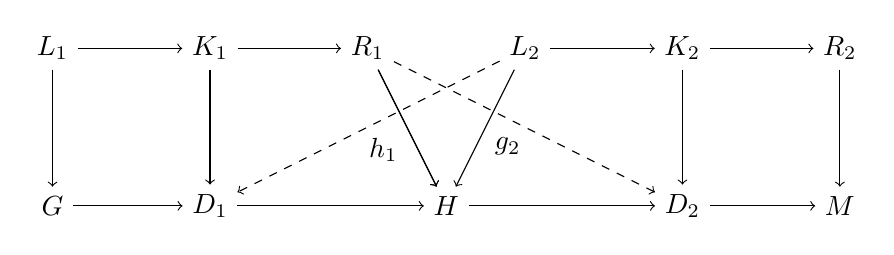
\begin{tikzpicture} 
        % Define nodes
        \node (L1) at (0,2) {$L_1$};
        \node (K1) at (2,2) {$K_1$};
        \node (R1) at (4,2) {$R_1$};
        \node (L2) at (6,2) {$L_2$};
        \node (K2) at (8,2) {$K_2$};
        \node (R2) at (10,2) {$R_2$};
        \node (G) at (0,0) {$G$};
        \node (T) at (5,0) {$H$};
        \node (M) at (10,0) {$M$};
        \node (D1) at (2,0) {$D_1$};
        \node (D2) at (8,0) {$D_2$};
      
        % Draw arrows
        % Top row
        \draw[->] (L1) -- node[above] {} (K1);
        \draw[->] (K1) -- node[above] {} (R1);
        \draw[->] (L2) -- node[above] {} (K2);
        \draw[->] (K2) -- node[above] {} (R2);
      
        % Vertical arrows
        \draw[->] (L1) -- node[left] {} (G);
        \draw[->] (R1) -- node[right] {} (T);
        \draw[->] (R2) -- node[right] {} (M);
        \draw[->] (K1) -- node[right] {} (D1);
        \draw[->] (K2) -- node[right] {} (D2);
      
        % Bottom row
        \draw[->] (G) -- node[below] {} (D1);
        \draw[->] (D1) -- node[below] {} (T);
        \draw[->] (T) -- node[below] {} (D2);
        \draw[->] (D2) -- node[below] {} (M);

        \draw[->,dashed] (R1) -- node[below] {} (D2);
        \draw[->,dashed] (L2) -- node[below] {} (D1);
      
        % Diagonal arrows
        \draw[->] (R1) -- node[below left] {$h_1$} (T);
        \draw[->] (L2) -- node[below right] {$g_2$} (T);
      \end{tikzpicture}
\end{definition}

\begin{definition}[Sequential critical pair]
    Let $r_i \colon \langle L_i \leftarrow K_i \rightarrow R_i \rangle$ be rules, for $i = 1, 2$. A pair of direct derivations $G \Rightarrow_{r_1} H \Rightarrow_{r_2} M$ as depicted below is a sequential critical pair if the following holds.
    \begin{itemize}
        \item Minimality:$H = h_1(R_1) \cup g_2(L_2)$.
        \item Conflict: The steps are not sequentially independent.
    \end{itemize}
    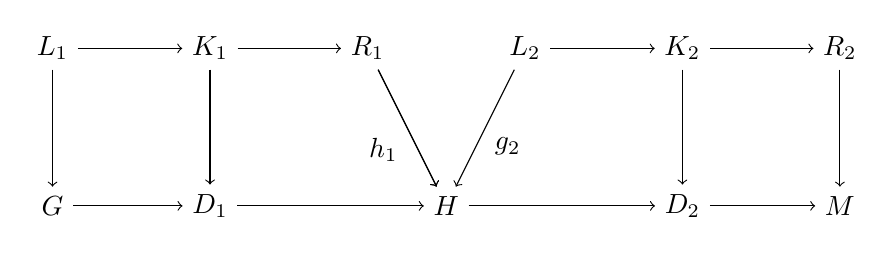
\begin{tikzpicture} 
        % Define nodes
        \node (L1) at (0,2) {$L_1$};
        \node (K1) at (2,2) {$K_1$};
        \node (R1) at (4,2) {$R_1$};
        \node (L2) at (6,2) {$L_2$};
        \node (K2) at (8,2) {$K_2$};
        \node (R2) at (10,2) {$R_2$};
        \node (G) at (0,0) {$G$};
        \node (T) at (5,0) {$H$};
        \node (M) at (10,0) {$M$};
        \node (D1) at (2,0) {$D_1$};
        \node (D2) at (8,0) {$D_2$};
      
        % Draw arrows
        % Top row
        \draw[->] (L1) -- node[above] {} (K1);
        \draw[->] (K1) -- node[above] {} (R1);
        \draw[->] (L2) -- node[above] {} (K2);
        \draw[->] (K2) -- node[above] {} (R2);
      
        % Vertical arrows
        \draw[->] (L1) -- node[left] {} (G);
        \draw[->] (R1) -- node[right] {} (T);
        \draw[->] (R2) -- node[right] {} (M);
        \draw[->] (K1) -- node[right] {} (D1);
        \draw[->] (K2) -- node[right] {} (D2);
      
        % Bottom row
        \draw[->] (G) -- node[below] {} (D1);
        \draw[->] (D1) -- node[below] {} (T);
        \draw[->] (T) -- node[below] {} (D2);
        \draw[->] (D2) -- node[below] {} (M);

        % \draw[->,dashed] (R1) -- node[below] {} (D2);
        % \draw[->,dashed] (L2) -- node[below] {} (D1);
      
        % Diagonal arrows
        \draw[->] (R1) -- node[below left] {$h_1$} (T);
        \draw[->] (L2) -- node[below right] {$g_2$} (T);
      \end{tikzpicture}
\end{definition}

\begin{theorem}
    \todo{rewrite}
    Let $\langle \Sigma, \mathcal{R} \rangle$ and $\langle \Sigma, \mathcal{S} \rangle$ be terminating hypergraph transformation systems. If there are no sequential critical pairs of shape $S \Rightarrow_{\mathcal{R}} T \Rightarrow_{\mathcal{S}} U$, then the combined system $\langle \Sigma, \mathcal{R} \cup \mathcal{S} \rangle$ is terminating.
\end{theorem}

% %     \subsection{Forward Closure Method of DPO GRS}  
% %     \label{sec:forward_closure}
% %     Plump \cite{Plump1995} introduced a necessary and sufficient termination condition for left-injective DPO hypergraph rewriting via forward closure, though verifying this condition is undecidable.


\begin{definition}[Instance]
    \todo{rewrite}
    Consider a finite or infinite derivation
    

    \begin{tikzpicture}
      % Nodes
      \node (pi1) at (0,0) {$\pi_1$};
      \node (pip1) at (2,0) {$\pi'_1$}; 
      \node (pi2) at (4,0) {$\pi_2$};
      \node (pip2) at (6,0) {$\pi'_2$};
      \node (pi3) at (8,0) {$\pi_3$};
      \node (pip3) at (10,0) {$\pi'_3$};
      \node (dots) at (12,0) {$\dots$};
    
      % Horizontal arrows in the top row
      \draw[->] (pi1) -- ++(-2,0);
      \draw[->] (pip1) -- ++(2,0);
      \draw[->] (pi2) -- ++(-2,0);
      \draw[->] (pip2) -- ++(2,0);
      \draw[->] (pi3) -- ++(-2,0);
      \draw[->] (pip3) -- ++(2,0);
    
      % Vertical arrows
      \draw[->] (pi1) -- ++(0,-1);
      \draw[->] (pip1) -- ++(0,-1);
      \draw[->] (pi2) -- ++(0,-1);
      \draw[->] (pip2) -- ++(0,-1);
      \draw[->] (pi3) -- ++(0,-1);
      \draw[->] (pip3) -- ++(0,-1);
    
      % Diagonal arrows
      \draw[->] (pip1) -- ++(1,-1);
      \draw[->] (pip2) -- ++(1,-1);
      \draw[->] (pip3) -- ++(1,-1);
    
      % Horizontal arrows in the bottom row
      \draw[->] (pi1) -- ++(2,0);
      \draw[->] (pip1) -- ++(-2,0);
      \draw[->] (pi2) -- ++(2,0);
      \draw[->] (pip2) -- ++(-2,0);
      \draw[->] (pi3) -- ++(2,0);
      \draw[->] (pip3) -- ++(-2,0);
    \end{tikzpicture}
    
    A derivation is an \textit{instance} (or \textit{embedding}) of this derivation if it can be written
    

    
    where for each $i \geq 1$, $\phi_i$ and $\phi'_i$ are pushouts with injective vertical morphisms. (So the pushouts constituting the derivation are composed of the pushouts $\pi_i$ and $\phi_i$, respectively $\pi'_i$ and $\phi'_i$.)
\end{definition}

\begin{definition}[forward closure]
    Forward closures are inductively defined as follows:
    \begin{enumerate}
        \item Every direct derivation $L \Rightarrow_{r,g} R$ with surjective $g$ is a forward closure.
        \item A derivation $G \Rightarrow^+ H \Rightarrow M$ is a forward closure if $G \Rightarrow^+ H$ is an instance of a forward closure, and $H \Rightarrow M$ is a direct derivation such that
        \begin{itemize}
            \item $G \Rightarrow^+ H$ and $H \Rightarrow M$ are dependent,
            \item $\text{New}(H) \subseteq \text{Redex}(H \Rightarrow M)$.
        \end{itemize}
    \end{enumerate}
\end{definition}

\begin{definition}[infinite forward closure]
    \todo{rewrite}
    An \textit{infinite forward closure} is an infinite derivation $G_0 \Rightarrow G_1 \Rightarrow G_2 \Rightarrow \dots$ that contains a forward closure as a prefix. That is, there is some $n \geq 1$ such that $G_0 \Rightarrow^+ G_n$ is a forward closure.
\end{definition}

\begin{definition}[Consumptive System]
    \todo{rewrite}
    A graph rewriting system is \textit{consumptive} if each rule $(L \leftarrow K \rightarrow R)$ has a non-surjective morphism $K \to L$.
\end{definition}
    
\begin{theorem}[Main Theorem]
    \todo{rewrite}
    A graph rewriting system is terminating if, and only if, it is consumptive and does not admit an infinite forward closure.
\end{theorem}
% %     \subsection{Termination Criterion of injective DPO GRS based on E-dependency relation \textcolor{red}{todo}} 
% \begin{definition}[E-graph]
\end{definition}

\begin{definition}[size of a graph]
\end{definition}

\begin{definition}[production]
\end{definition}

\begin{definition}[E-concurrent production~\text{\cite[Def~3.1]{LEVENDOVSZKY200787}}]
    An E-concurrent production $p^*$ is an E-based composition if there is at least one input graph $G_0$ with an E-related transformation $G_0 \xrightarrow{p^*} H$.
\end{definition}

\begin{definition}[E-dependency relation~\text{\cite[Def~3.2]{LEVENDOVSZKY200787}}]
    Consider a possibly infinite sequence of graph productions $p_i$, ($i \mathop{=} 1, 2, \ldots$) and a sequence of E-dependency relations $((E_i, e_i^*, e_{i+1}))$ leading to a sequence of their E-based compositions $(p_i^* \mathop{=} (L_i^* \mathop{\leftarrow} K_i^* \mathop{\rightarrow} R_i^*))$ with $p_1^* \mathop{=} p_1$ and $p_n^* \mathop{=} (p_1 *_{E_1} p_2) *_{E_2} \ldots *_{E_n} p_n$.
    
    A cumulative LHS series of this sequence is the graph series $L_n^*$ consisting of the left-hand side graphs of $p_n^*$. Moreover, a cumulative size series of a production sequence is the nonnegative integer series $|L_n^*|$.
    \end{definition}

\begin{theorem}[Termination~\cite{LEVENDOVSZKY200787}]
    A \text{GTS} $= (P)$ (Def.??) terminates if for all infinite cumulative LHS sequences $(L_i^*)$ of the graph productions created from the members of $P$, it holds that
    \[
    \lim_{i \mathop{\to} \infty} |L_i^*| \mathop{=} \infty.
    \]
    Note that we assume finite input graphs and injective matches.
\end{theorem} 
%     \subsection{Type Graph Method for DPO GRS}
%     \label{sec:type_graph_method}
%         \subsubsection{Well-founded semirings}
%         \begin{definition}[Monoid]
    \label{def:monoid}
    \todo{to check and add reference}
    A \textbf{monoid} is a triple \(\langle S, \cdot, e \rangle\) where \(S\) is a set, \(\cdot : S \times S \to S\) is a binary operation and \(e \in S\) is constant
    satisfying for all \(a, b, c \in S\):
    \begin{itemize}
        \item \textbf{Associativity}: \((a \cdot b) \cdot c = a \cdot (b \cdot c)\),
        \item \textbf{Identity}: \(a \cdot e = a = e \cdot a\).
    \end{itemize}
    The monoid is \textbf{commutative} if \(a \cdot b = b \cdot a\) for all \(a, b \in S\).
\end{definition} 

\begin{definition}[Semiring]
    \label{def:semiring}
    \todo{to check and to add some references}
    A \textbf{semiring} is a tuple \(\langle S, \oplus, \odot, 0, 1 \rangle\) where:
    \begin{itemize}
        \item  \(\langle S, \oplus, 0 \rangle\) forms a commutative monoid,
        \item  \(\langle S, \odot, 1 \rangle\) forms a monoid,
        \item  $0$ is an annihilator for $\odot$ : For all \(a \in S\),
              \(
                  0 \odot a = 0 = a \odot 0
              \),
        \item $\odot$ distributes over $\oplus$: For all \(a, b, x \in S\),
              \begin{itemize}
                \item $(a \oplus b) \odot x = (a \odot x) \oplus (b \odot x)$
                \item $x \odot (a \oplus b) = (x \odot a) \oplus (x \odot b)$
              \end{itemize}                 
    \end{itemize}
    The semiring is \textbf{commutative} if its multiplicative monoid \(\langle S, \odot, 1 \rangle\) is commutative.
\end{definition}


\begin{definition}[Well-founded semiring]
    \label{def:well_founded_semiring}
    A \textbf{well-founded semiring} is a tuple \(\langle S, \oplus, \odot, 0, 1, \prec, \leq \rangle\) where:
    \begin{itemize}
        \item  \(\langle S, \oplus, \odot, 0, 1 \rangle\) is a semiring,
        \item \textbf{Order Relations}: 
            \begin{itemize}
                \item \(\prec, \leq \subseteq S \times S\) are non-empty orders,
                \item \(\prec \subseteq \leq\) (i.e., \(x \prec y \implies x \leq y\)),
                \item \(\leq\) is reflexive.
            \end{itemize}
    \end{itemize}
    The structure satisfies:
    \begin{itemize}
        \item \(\text{SN}(\succ / \geq)\) (strong normalization modulo \(\geq\)),
        \item \(0 \neq 1\),
        \item For all \(x, x', y, y' \in S\):
            \begin{align*}
                x \leq x' \land y \leq y' &\implies x \oplus y \leq x' \oplus y' \tag{S1} \label{ax:S1} \\
                x \prec x' \land y \prec y' &\implies x \oplus y \prec x' \oplus y' \tag{S2} \label{ax:S2} \\
                x \leq x' \land 1 \leq y &\implies x \odot y \leq x' \odot y \tag{S3} \label{ax:S3} \\
                x \prec x' \land 1 \leq y \neq 0 &\implies x \odot y \prec x' \odot y \tag{S4} \label{ax:S4}
            \end{align*}
    \end{itemize}
    The semiring is \textbf{strictly monotonic} if it additionally satisfies:
    \[
        x \prec x' \land y \leq y' \implies x \oplus y \prec x' \oplus y' \tag{S5} \label{ax:S5}
    \]
\end{definition}

\begin{example}[Semiring examples~\text{\cite[Ex. 2.7]{endrullis2024generalized}}]
    \label{ex:semiring_examples}
    \textbf{Arithmetic semiring}: \(\langle \mathbb{N}, +, \cdot, 0, 1, <, \leq \rangle\) is strictly monotonic and well-founded.

    \textbf{Tropical semiring}: \(\langle \mathbb{N} \cup \{\infty\}, \min, +, \infty, 0, <, \leq \rangle\) is well-founded but not strictly monotone.

    \textbf{Arctic semiring}: \(\langle \mathbb{N} \cup \{-\infty\}, \max, +, -\infty, 0, <, \leq \rangle\) is well-founded but not strictly monotone.
\end{example}
%         \subsubsection{Weighted Type Graphs}
%         The following definition of a weighted type graph is obtained from~\cite[\textdef~3.1]{endrullis2024generalized}.
\begin{definition}[Weighted Type Graph]
    \label{def:weighted_type_graph}
    A \textbf{weighted type graph} \(\mathcal{T} \mathop{=} (T, \mathbb{E}, \mathcal{S}, w)\) consists of:
    \begin{itemize} 
        \item An object \(T \mathop{\in} \mathcal{C}_0\), called the \textbf{type graph},
        \item A set \(\mathbb{E}\) of arrows \(e \mathop{\in} \mathcal{C}_1\) with \(\operatorname{codom}(e) \mathop{=} T\), called the \textbf{\(T\)-valued elements},
        \item A well-founded, commutative semiring \(\mathcal{S}=\langle S, \mathop{\oplus}, \mathop{\odot}, 0, 1, \prec, \leq \rangle \),
        \item A weight function \(w : \mathbb{E} \mathop{\to} S \mathop{\setminus} \{0_S\}\).
    \end{itemize}
    \(\mathcal{T}\) is \textbf{finitary} if for every \((e:X \mathop{\to} T) \mathop{\in} \mathbb{E}\) and every \(G \mathop{\in} \mathcal{C}_0\), the sets \(\operatorname{Hom}(X, G)\) and \(\operatorname{Hom}(G, T)\) are finite.
\end{definition}
\todo{include : $weighted_type_graph_remark_geq1$}
\todo{include : $weighted_type_graph_remark_neq0$}
%         \subsubsection{Weighing Morphisms and Objects}
%         % \begin{notation} For morphisms \( \alpha : A \to B \), \( \beta : B \to C \), \( \gamma : A \to C \) and $E \subseteq \operatorname{Hom}(A,B)$, define:
%     \begin{flalign*}
%                \set{ \alpha \star - = \gamma } &\overset{\operatorname{def}}{=} \{ \beta \in \operatorname{Hom}(B, C) \mid \alpha \star \beta = \gamma \}.
%    \\
%                \set{ - \star \beta = \gamma }  &\overset{\operatorname{def}}{=} \{ \alpha \in \operatorname{Hom}(A, B) \mid \alpha \star \beta = \gamma \}.
%    \\
%                E \star \beta                   &\overset{\operatorname{def}}{=} \set{ \alpha \star \beta \mid \alpha \in E }.
%     \end{flalign*}
%    \end{notation} 
   
   \begin{definition} 
       \label{def:bigodot}
   Let $(S, \oplus, \odot, 0_s, 1_s)$ be a semiring. We define 
    \begin{flalign*}
       \bigodot \emptyset &\overset{\operatorname{def}}{=} 1_s
   \\
       \bigodot \left( E \cup \{x\} \right) &\overset{\operatorname{def}}{=} \left( \bigodot E \right) \odot x
       \\
       \bigoplus \emptyset &\overset{\operatorname{def}}{=} 0_s
       \\
           \bigoplus \left( E \cup \{x\} \right) &\overset{\operatorname{def}}{=} \left( \bigoplus E \right) \oplus x
   \end{flalign*}
   \end{definition}
    
   
   \begin{definition}[\text{\cite[\textdef~3.4]{endrullis2024generalized}}] 
       \label{def:weight}
       Let $\mathcal{T} = (T,\mathbb{E},S, w)$ be a finitary type
       \newline
       \noindent
       \begin{minipage}{0.6\textwidth}graph.~The \textbf{weight of a morphism $h: G \rightarrow T$ relative to $(e:X \to T) \in \mathbb{E}$} is defined as the weight $w(e)$ raised to the power of the number of $\iota$ making the diagram (shown on the right) commutative.
       \end{minipage}
       \begin{minipage}{0.29\textwidth}
           \begin{center}
                   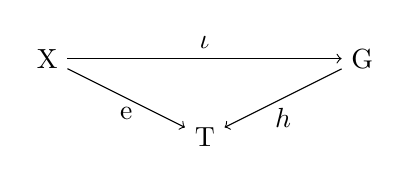
\begin{tikzpicture}
                       \node (a) at (0,0) {X};
                       \node (c) at (4,0) {G};
                       \node (d) at (2,-1) {T};
                       \draw[->] (a) -- (d) node [midway,below] {e};
                       \draw[->] (a) -- (c) node [midway,above] {$\iota$};
                       \draw[->] (c) -- (d) node[midway, below] {$h$};
                       % \node (d) at (2,-0.5) {=};
                   \end{tikzpicture}
           \end{center} 
       \end{minipage}
                   \[
                   w_e(h) 
                       \overset{\operatorname{def}}{=}
                   \underset{\alpha \in \{- \star h = e\}}{\bigodot}w(e) 
                   \]
           % which can be visualized as $w(e)$ raised to the power of the number of possible morphisms $g$ which make the following commutative diagram hold
   
           \noindent
           The \textbf{weight of a morphism $h: G \rightarrow T$ relative to \(\mathcal{T}\)} is defined as the semiring product of $w(e)$ for $e \in \mathbb{E}$:
           \[  w_\mathcal{T}(h) \overset{\operatorname{def}}{=} \underset{e \in \mathbb{E}}{\bigodot} 
                   w_e(h) \]
   
           \noindent
          The \textbf{weight of an object \( G \in \mathcal{C}_0 \) relative to \( \mathcal{T}\)} is defined as the semiring sum of $w_\mathcal{T}(h)$ for $h \in \operatorname{Hom}(G,T)$:
           \[w_\mathcal{T}(G) \overset{\operatorname{def}}{=} \underset{h \in \operatorname{Hom}(G,T)}{\bigoplus}  w_\mathcal{T}(h) \]
   \end{definition}
   
   
   % In certain scenarios, we want to exclude specific morphisms when calculating morphism weight relative to a give T-valued element $e:X \to T$. For this reason, for all set \( \Gamma \subseteq \operatorname{Hom}(A, G) \), we define 
   
   
   
   % The weight of the morphism \( \phi : G \to T\) excluding morphisms in \( \Gamma' \) is defined as the number of morphisms from \( X \) to \( G \) that do not factor through any \( \alpha \in \Gamma \).
   
   \begin{definition}[\text{\cite[\textdef~3.4]{endrullis2024generalized}}]
       \label{def:weight_excluding}
       Let \( A \in \mathcal{C}_0 \) and $\Gamma \subseteq \operatorname{Hom}(A,G)$. We de-
       \newline
       \noindent
       \begin{minipage}{0.6\textwidth}
         fine $\Gamma'$ as the set consisting of all morphisms \( \iota : X \to G \) admitting morphisms \( \zeta \colon X \to A \) and \( \alpha \in \Gamma \) such that the diagram illustrated on the right is commutative. Formally, 
       \end{minipage}
       \begin{minipage}{0.4\textwidth}
           \hfill 
           % \begin{center}
               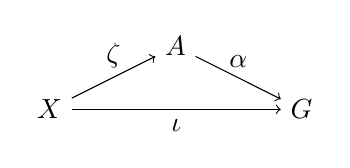
\begin{tikzpicture}[scale=0.8]
                   \node (X) at (0,0) {\(X \)};
                   \node (A) at (2,1) {\( A \)};
                   \node (G) at (4,0) {\( G \)}; 
                   \draw[->] (X) -- (A) node[midway, above] {\( \zeta \)};
                   \draw[ ->] (X) -- (G) node[midway, below] {\( \iota \)};
                   \draw[->] (A) -- (G) node[midway, above] {\( \alpha \)};
                   % \node at (2,0.5) {\( = \)};
                   % \node (T) at (2,-1) {\( T \)};
                   % \draw[ ->] (X) -- (T) node[midway, below] {e};
                   % \draw[<-] (T) -- (G) node[midway, above] {};
               \end{tikzpicture}
           % \end{center} 
       \end{minipage}
   
       \[
       \Gamma' \overset{\operatorname{def}}{=} \left\{ \iota \in \operatorname{Hom}(X, G)~\middle|~\exists \alpha \in \Gamma,~\exists \zeta:X \to A,~\zeta \star \alpha = \iota \right\}.
       \]
   
       \noindent
       The \textbf{weight of a morphism \(h : G \to T\) excluding morphisms in \( \Gamma' \) relative to $(e:X \to T) \in \mathbb{E}$} is defined as $w(e)$ raised to the power of the number of morphisms \( (\iota : X \to G) \notin \Gamma' \).
           \[
           w_e(h - \Gamma) \overset{\operatorname{def}}{=} \underset{
               \substack{\alpha \in \set{- \star h = e} \\
                           \alpha \notin \Gamma'}}{\bigodot} w(e)\] 
           The \textbf{weight of a morphism $h: G \to T$ excluding morphisms in \( \Gamma' \) relative to \(\mathcal{T}\)} is defined as the semiring product of $w_e(h-\Gamma)$ for $e \in \mathbb{E}$:
           \[ 
               w_\mathcal{T}(h-\Gamma) \overset{\operatorname{def}}{=} \underset{e \in \mathbb{E}}{\bigodot} 
           w_e(h-\Gamma)
                   \]
   \end{definition} 
   % \begin{definition}[Weight excluding morphisms \cite{endrullis2024generalized}]
   %     \label{def:weight_excluding}
   %     Let \(\Gamma \subseteq \operatorname{Hom}(A, G)\). Define:
   %     \[
   %     \Gamma' \overset{\text{def}}{=} \left\{ \iota \in \operatorname{Hom}(X, G) \,\middle|\, \exists \alpha \in \Gamma, \exists \zeta : X \to A, \, \zeta \star \alpha = \iota \right\}.
   %     \]
   %     The \textbf{weight of \(h : G \to T\) excluding \(\Gamma'\)} is:
   %     \[
   %     w_e(h - \Gamma) \overset{\text{def}}{=} \bigodot_{\substack{\iota \in \{- \star h = e\} \\ \iota \notin \Gamma'}} w(e), \quad
   %     w_\mathcal{T}(h - \Gamma) \overset{\text{def}}{=} \bigodot_{e \in \mathbb{E}} w_e(h - \Gamma).
   %     \]
   % \end{definition}
       If \( \Gamma \) is a singleton \( \{ \alpha \} \), we denote \( w_{\mathcal{T}_\Sigma^X}(h - \alpha) \) instead of \( w_{\mathcal{T}_\Sigma^X}(h - \{ \alpha \}) \).
%         \subsubsection{Estimating Weight Changes}
%         In this section, we recall the concepts of traceability, relative monicity and weighable pushout square. These concepts are used to constrain \(T\)-valued elements and the DPO rewriting framework.  
For further details, we refer the reader to \cite[Section 4.1 and 4.2]{endrullis2024generalized}.
\begin{definition}[Traceability~\text{\cite[\textdef~4.1]{endrullis2024generalized}}]
    \label{def:traceability}
    \ \newline
\noindent 
\begin{minipage}{0.5\textwidth}
An object $X \mathop{\in} \mathcal{C}$ is called \emph{traceable} along a class of pushout squares $\Delta$ if for every diagram $\delta \mathop{\in} \Delta$ (shown on the right), the following hold
\end{minipage}
\begin{minipage}{0.5\textwidth}
\begin{center}
    \begin{tikzpicture}[node distance=12mm]
      \node (A) {$A$};
      \node [right of=A] (B) {$B$}; 
      \node [below of=A] (C) {$C$}; 
      \node [below of=B] (D) {$D$}; 
      \node [right of=D] (X) {$X$};
      \begin{scope}[nodes=rectangle]          
      \draw [->] (A) to node [above,label,pos=0.5] {$\alpha$} (B);
      \draw [->] (A) to node [left,label,pos=0.5] {$\beta$} (C);
      \draw [->] (B) to node [right,label,pos=0.45] {$\beta'$} (D); 
      \draw [->] (C) to node [below,label,pos=0.45] {$\alpha'$} (D);
      \draw [->] (X) to node [below,label,pos=0.4] {$f$} (D);
      \end{scope}
      \node at ($(A)!.5!(D)$) {$\delta$};
    \end{tikzpicture}
\end{center}
\end{minipage}
    \begin{enumerate}[label=(\alph*)]
        \item\label{traceable:a} there exists a morphism $h : X \mathop{\to} B$ such that $f \mathop{=} h \mathop{\star} \beta'$, or
        \item\label{traceable:b} there exists an $h : X \mathop{\to} C$ such that $f \mathop{=} h \mathop{\star} \alpha'$.
    \end{enumerate}
    If additionally, 
    \textcolor{red}{whenever \ref{traceable:a} and \ref {traceable:b} hold,} \todo{This starts to be quite hard to follow without intuition or example}
    \begin{enumerate}[label=(\alph*),resume]
        \item 
        there exists a morphism $h : X \mathop{\to} A$ such that $f \mathop{=} h \mathop{\star} \alpha \mathop{\star} \beta' $,
    \end{enumerate}
    then we say that $X$ is \emph{strongly traceable} along $\Delta$.
\end{definition}
\begin{definition}[Relative Monicity~\text{\cite[\textdef~4.6]{endrullis2024generalized}}]
    Let $A,B,C$ and $X$ be objects, $\Gamma$ a set of objects, $S$ a set of morphisms to $A$ and $u:C\to A$ a morphism. A morphism $f : A \to B$ is called 
    \begin{enumerate}[label=(\roman*)] 
        \item 
            \emph{monic for $S$} 
            if $g \star f = h \star f$ implies $g = h$ for all $g, h \in S$;
        \item 
            \emph{$X$-monic} if $f$ is monic for $\operatorname{Hom}(X, A)$.
        \item \emph{$X$-monic outside of $u$}, if $f$ is monic for \( \operatorname{Hom}(X,A) \setminus \left ( \operatorname{Hom}(X,C) \star u \right ) \).
        \item  \emph{$\Gamma$-monic} if $f$ is $X$-monic for every $X \in \Gamma$.
    \end{enumerate}
\end{definition} 
\begin{definition}[Weighable Pushout Square~\text{\cite[\textdef~4.9]{endrullis2024generalized}}]
    \label{def:weighable}
    \ \newline
    \noindent
    \begin{minipage}{0.7\textwidth}
        Let  $\mathcal{T} = (T,\mathbb{E}, S, w)$ be a finitary weighted type graph.
        Consider the pushout square $\delta$ shown on the right. We say that $\delta$ is
    \end{minipage}
    \begin{minipage}{0.3\textwidth}
        \begin{center}
            \begin{tikzpicture}[node distance=12mm]
                \node (A) {$A$};
                \node (B) [right of=A] {$B$};
                \node (C) [below of=A] {$C$};
                \node (D) [right of=C] {$D$};
                \draw [->] (A) to node [above, label] {$\alpha$} (B);
                \draw [->] (A) to node [left, label] {$\beta$} (C);
                \draw [->] (B) to node [right, label] {$\beta'$} (D);
                \draw [->] (C) to node [below, label] {$\alpha'$} (D);
                \node [at=($(A)!.5!(D)$)] {$\delta$};
            \end{tikzpicture}
        \end{center}
    \end{minipage}
    \begin{enumerate}[label=(\alph*)]
        \item \emph{weighable} with $\mathcal{T}$ if the following hold:
            \begin{enumerate}[label=(\roman*)]
                \item $dom(\mathbb{E})$ is strongly traceable along $\delta$,
                \item $\beta'$ is $dom(\mathbb{E})$-monic,
                \item $\alpha'$ is $dom(\mathbb{E})$-monic outside of $\beta$.
            \end{enumerate}
        \item \emph{bounded-above} by $\mathcal{T}$ if $dom(\mathbb{E})$ is traceable along $\delta$.
    \end{enumerate}
\end{definition}
The existence of a context closure guarantees the existence of morphisms from any object subject to rewriting to the type graph—a critical requirement as emphasized in \hyperref[remark:semiring_0_unpredictable]{\textsection~\ref{remark:semiring_0_unpredictable}}. Further details can be found in~\cite[\textsection 5.3]{endrullis2024generalized}.
\begin{definition}[Context Closure~\text{\cite[\textdef~5.3]{endrullis2024generalized}}]
    \label{def:context_closure} 
    \ \newline 
\begin{minipage}{0.65\textwidth}
    Let $\mathcal{T} = (T,\mathbb{E}, S, w)$ be a type graph, \(\rho = (L \overset{l}{\leftarrow} K \overset{r}{\rightarrow} R ) \) a DPO rewriting rule and $\mathfrak{F}$ a rewriting framework. 
    A \textbf{context closure} for $\rho$ and $\mathcal{T}$ in $\mathfrak{F}$ is a morphism $c:L \rightarrow T$ such that for every DPO diagram in $\mathfrak{F}(\rho)$ (shown on the right) 
    there exists $\alpha : G \rightarrow T$ such that $m \star \alpha = c$.
\end{minipage}
\begin{minipage}{0.35\textwidth}
    \begin{center}
        \begin{tikzpicture}[rotate=90]
          \node (I) {$K$}; 
          \node (L) [left of=I] {$L$};
          \node (R) [right of=I] {$R$};
          \node (G) [below of=L] {$G$};
          \node (C) [below of=I] {$C$};
          \node (H) [below of=R] {$H$};
          \node (T) [left=of $(L)!0.5!(G)$] {$T$};
          \draw [->] (L) to  node [label, above] {$c$}  (T);
          \draw [->] (G) to  node [label, below] {$\alpha$} (T);
          \draw [->] (I) to node [label, above] {$l$} (L);
          \draw [->] (I) to node [label,above] {$r$} (R);
          \draw [->] (L) to node [label, right] {$m$} (G);
          \draw [->] (I) to (C);
          \draw [->] (R) to (H);
          \draw [->] (C) to (G);
          \draw [->] (C) to (H);
        \end{tikzpicture}
      \end{center}
\end{minipage}
\end{definition}
%         % \subsection{Decreasing Rule}
%         \todo{to be weakened to the original version by endrullis}
\todo{maybe add the core lemma for estimating pushout object weight, but adapt to estimating DPO objects weight difference}
\begin{definition}[Decreasing Rules~\text{\cite[\textdef~5.9]{endrullis2024generalized}}]
    \label{def:decreasing_rule}
    Let $\mathcal{T} = (T,\mathbb{E},\mathcal{S}, w)$ be a finitary weighted type graph where $\mathcal{S}=\langle S, \oplus, \odot, 0, 1, \prec, \leq \rangle$ is a well-founded, commutative, \(\mathfrak{F}\) a DPO rewriting framework, $\rho = (L \overset{l}{\leftarrow} K \overset{r}{\rightarrow} R)$ a DPO rewriting rule. 

    \noindent
    The rule $\rho$ is \textbf{weakly decreasing} w.r.t. $\mathcal{T}$ in $\mathfrak{F}$ if 
            for every $t_K : K \to T$,
                $$ 
                  w_\mathcal{T}(\{l \star - = t_K\}) \succeq w_\mathcal{T}(\{r\star - = t_K\})$$
           
    \noindent
    The rule $\rho$ is \textbf{uniformly decreasing} w.r.t. $\mathcal{T}$ in $\mathfrak{F}$ if
        \begin{itemize}
            \item[]- there exists a context closure $c_\rho$ for $\rho$ and $\mathcal{T}$ in $\mathfrak{F}$, and
            \item[]- for every $t_K : K \to T$,
            \begin{itemize}
                \item[] $\bullet$ $\{l \star - = t_K\} = \emptyset = \{r \star - = t_K\}$, or
                \item[] $\bullet$ $w_\mathcal{T}(\{l \star - = t_K\}) \succ    w_\mathcal{T}(\{r \star - = t_K\}) + \delta$.
            \end{itemize}
        \end{itemize}  
         
    \noindent
    The rule $\rho$ is
            \textbf{$\delta$-closure decreasing} w.r.t. $\mathcal{T}$ in $\mathfrak{F}$ if the following hold:
            \begin{itemize}
                \item[]- $S$ is strictly monotonic semiring,
                \item[]- $\rho$ is weakly decreasing,
                \item[]- there exists a context closure $c_\rho$ for $\rho$ and $\mathcal{T}$ in $\mathfrak{F}$,
                \item[]- $w_\mathcal{T}(\{l \star - = t_K\}) \succ  w_\mathcal{T}(\{r \star - = t_K\})$ for $t_K = l \star c_\rho$.
            \end{itemize}
\end{definition}

The following lemma states that decreasing rules reduce the weights of host graphs, provided specific constraints are satisfied.
\begin{lemma}[Decreasing steps~\text{\cite[Theorem C.3]{endrullis2024generalized}}]
    \label{lem:decreasing_step}
    \ \newline 
\begin{minipage}{0.7\textwidth}
    Let $\mathcal{T} = (T,\mathbb{E}, \mathcal{S}, w)$ be a finitary weighted type graph where $\mathcal{S} = \langle S, \oplus, \odot, 0, 1, \prec, \leq \rangle$ is a strong monotonic, commutative semiring, $\rho$ a rewriting rule and $\Delta \in \mathfrak{F}(\rho)$ a DPO diagram
    (shown on the right)   such that the following conditions hold:
\end{minipage}  
\begin{minipage}{0.3\textwidth}
    \begin{center}
        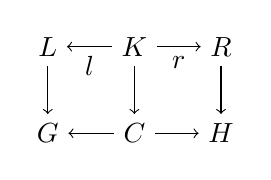
\begin{tikzpicture}[node distance=11mm]
          \node (I) {$K$};
          \node (L) [left of= I] {$L$};
          \node (R) [right of=I] {$R$}; 
          \node (G) [below of=L] {$G$};
          \node (C) [below of=I] {$C$};
          \node (H) [below of=R] {$H$};
        %   \node (T) [left=of $(L)!0.5!(G)$] {$T$};
        %   \draw [->] (L) to  node [label, above] {$c$}  (T);
        %   \draw [->] (G) to  node [label, below] {$\alpha$} (T);
          \draw [->] (I) to node [label, below] {$l$} (L);
          \draw [->] (I) to node [label, below] {$r$} (R);
          \draw [->] (L) to  (G);
          \draw [->] (I) to (C);
          \draw [->] (R) to (H);
          \draw [->] (C) to (G);
          \draw [->] (C) to (H);
        \end{tikzpicture}
      \end{center}
\end{minipage}
   \begin{itemize}
       \item $\operatorname{left}(\Delta)$ is weighable with \(\mathcal{T}\), and
       \item $\operatorname{right}(\Delta)$ is bounded above by \(\mathcal{T}\), and
       \item $w(e) \succeq 1_S$ for all $e \in \mathbb{E}$.
   \end{itemize}

   \noindent
  We have:
   \begin{itemize}
       \item $w_\mathcal{T}(G) \succeq w_\mathcal{T}(H)$ if $\rho$ is weakly decreasing,
       \item $w_\mathcal{T}(G) \succ w_\mathcal{T}(H)$ if $w(e) \succeq 1_S$ for all $e \in \mathbb{E}$, and $\rho$ is uniformly or closure decreasing.
   \end{itemize}
\end{lemma} 
\begin{proof}
   See the \hyperref[proof:decreasing_step]{Appendix}.
\end{proof} 
%         \subsubsection{Termination Criterion} 
%         \todo{to be weakened to the original version by endrullis}
Finally, a termination criterion can be established.
\begin{theorem}[Termination~\text{\cite[Theorem 5.11]{endrullis2024generalized}}] 
    \label{thm:termination_grs}
    Let $\mathcal{A}$ and $\mathcal{B}$ be sets of DPO rewriting rules, $\mathcal{T} \mathop{=} (T,\mathbb{E}, \mathcal{S}, w)$ be a finitary weighted type graph where $\mathcal{S} \mathop{=} \langle S, \mathop{\oplus}, \mathop{\odot}, 0, 1, \prec, \leq \rangle$ is a strong monotonic, commutative semiring and $\mathfrak{F}$ a DPO rewriting framework such that

     \begin{enumerate}
        \item\label{thm1:hyp3} $w(e) \mathop{\succeq} 1_S$ for all $e \mathop{\in} \mathbb{E}$,
        % \item\label{thm1:hyp4} $\{s \mathop{\in} S\mid 1_S \leq s \mathop{\neq} 0_S\} \mathop{\subseteq} \mathbb{R}_{>0}$ 
        % \item\label{thm1:hyp4} for all $x \mathop{\in} S$, if $ 1_S \mathop{\preceq} x \mathop{\neq} 0_S$ then $\mu(x) \mathop{\geq} \mu(1_S)$ and $\mu(x) \mathop{\in} \mathbb{R}$,
        % \item\label{thm1:hyp4} for all $x \mathop{\in} S$, if $ 1_S \mathop{\preceq} x \mathop{\neq} 0_S$ then $\mu(x) \mathop{\geq} \mu(1_S)$ and $\mu(x) \mathop{\in} \mathbb{R}$,
        \item for every rule $\rho \mathop{\in} (\mathcal{A }\mathop{\cup} \mathcal{B })$ and every double pushout diagram  
        $\Delta \mathop{\in} \mathfrak{F}(\rho)$ 
        \begin{itemize}
            \item \(\operatorname{left}(\Delta)\) is weighable with \(\mathcal{T}\), and
            \item \(\operatorname{right}(\Delta)\) is bounded above by \(\mathcal{T}\). 
        \end{itemize}
    \end{enumerate}       

    \noindent If the following conditions hold:
    \begin{enumerate}
        \item either every $\rho \mathop{\in} \mathcal{A}$ is uniformly decreasing, or every $\rho \mathop{\in} \mathcal{A}$ is closure decreasing,
        \item every rule $\rho \mathop{\in} \mathcal{B}$ is weakly decreasing,
    \end{enumerate}
    then $\mathop{\Rightarrow}_{\mathcal{A},\mathfrak{F}}$ is \textbf{terminating} relative to $\mathop{\Rightarrow}_{\mathcal{B},\mathfrak{F}}$.
\end{theorem} 
\begin{proof}
    See the 
    % \hyperref[proof_termination_grs]{Appendix}.
    ref
\end{proof}
%     \subsection{Subgraph Counting}  
%     The subgraph-counting method in 2024 lmcs by Overbeek and Endrullis is designed for the PBPO+ 2023 pbpo+ ref —a rewriting formalism capable of simulating left-injective DPO rewriting.
%     \subsection{Termination Criterion for DPO GRS with NAC}
%     \begin{definition}
    Let $V_L$ be the set of nodes in $L$, and $M_L \mathop{=} \{m_1, \dots, m_r\}$ the set of matches $m_i : V_L \mathop{\to} V_L$ of $V_L$ into itself, including the identity $id_{V_L} \mathop{=} m_1$. We construct a Labelled Transition System $\mathcal{L}^p \mathop{=} (S, \Lambda, \longrightarrow)$ as follows:

    \begin{enumerate}
        \item $S$ contains a state $s_i$ for each graph 
        $H_i^p \mathop{\in} \mathfrak{H}_p^p$. 
        % $H_i^p \mathop{\in} \mathscr{H}$.
         Each $s_i$ induces a classification function $c_i$ for matches of $p$ such that $c_i(m_l) \mathop{=} \text{true}$ iff $m_l$ can be extended to a match on $H_i^p$, but not to a match on any other 
         $H_j^p \mathop{\in} \mathfrak{H}_p^p \mathop{\setminus} (\{H_1^p, H_i^p\} \mathop{\cup} \{H_t^p \mid \exists h_t^i : H_t^p \mathop{\to} H_i^p\})$,
          i.e., $H_i^p$ is the biggest graph to which $m_l$ can be extended.
        
        \item $\Lambda$ contains a label $p^i$, $i \mathop{=} 1, \dots, r$ for each morphism in $M_L$.
        
        \item The transition relation $\longrightarrow \mathop{\subseteq} S \mathop{\times} \Lambda \mathop{\times} S$ is such that $(s_i, p^l, s_j) \mathop{\in} \longrightarrow$ (denoted by $s_i \xrightarrow{p^l} s_j$) if applying $p$ with match $m_l$ on graph $H_i^p$ produces a graph for which $c_j(m_l) \mathop{=} \text{true}$.
    \end{enumerate}
\end{definition} 

\begin{definition}
    In order to consider the variation on the number of possible matches induced by the application of $p$ on the minimal context for a given state, let $@|\cdot|: S \mathop{\to} \mathbb{N}$ be a function which associates with each state $s_i$ the number of matches for $p$ on the graph $H_i^p$ prior to application of $p$, and with $|\cdot|: S \mathop{\to} \mathbb{N}$ the function defining the number of matches on $H_i^p$ after the application of $p$.
\end{definition}

\begin{definition}
    Let $\rho$ be a graph rewriting rule. We say that $\rho$
    \begin{itemize}
        \item \emph{must terminate} if it should terminate simply and for all transitions $s_i \xrightarrow{p_l} s_j$ and all states $s_h \mathop{\neq} s_i, s_j, s_k$, we have $\left| s_i \right| < @ | s_i |$, $\left| s_j \right| \leq @ | s_j |\mathop{+}1$ and $\left| s_h \right| \leq @ | s_h |$.
        \item \emph{may terminates} if it may terminate simply and for all states on the path the same condition on matches as above applies.
        \item \emph{does not terminate} if (it does not terminate simply AND for all states from which $s_k$ is reachable, there is a state for which the number of matches increases for some transition leading to $s_k$ increases) OR (it should or may terminate simply, but there is at least one state $s_i$ on a path from $s_1$ to $s_k$ for which $\left| s_i \right| \mathop{\geq} @ | s_i |$, for a transition reachable from state $s_i$).
    \end{itemize}
\end{definition}

\begin{theorem}[Termination~\text{\cite[Theorem~2]{bottoni2010atermination}}]
    \todo{rewrite}
    Let $@|\cdot|: S \mathop{\to} \mathbb{N}$ and $|\cdot|: S \mathop{\to} \mathbb{N}$ be counting functions as defined above, let $p$ be a rule, and let $G$ be a finite graph. Then the following holds:
    \begin{enumerate}
        \item If rule $p$ is of type \textbf{must terminate}, then the application of \texttt{asLongAsPossible $p$ end} on the starting graph $G$ terminates after a finite number of steps.
        
        \item If $p$ is of type \textbf{does not terminate}, then the application of \texttt{asLongAsPossible $p$ end} on the starting graph $G$ does not terminate.
    \end{enumerate}
\end{theorem}   
\section{Morphisms of Graph Rewriting Systems}
    \label{sec:morphisms_from_dpo_to_pbpop}
    \subsection{Morphism from left-injective DPO GRS with injective match to PBPO+}
    \label{sec:morphism_from_dpo_grs_to_pbpop}
    \begin{example}[ \cite{overbeek2023pbpo_JLAMP}]
        In the category of unlabeled directed graphs, there exists a mono-partial morphism classifier $(T,\eta)$ where 
        \begin{itemize}
            \item for all unlabeled graph $G=(V,A,s,t)$, we have $T(G) \mathop{=} (V_*,E_*,s_*,t_*)$ where $V_* \mathop{=} V \uplus \{*\}, E_* \mathop{=} E \uplus (V_* \mathop{\times} V_x), s_*(e) \mathop{=} s(e)$ if $e \mathop{\in} E$ and $\pi_1(e)$ otherwise, and $t_*(e) \mathop{=} t(e)$ if $e \mathop{\in} E$ and $\pi_2(e)$ otherwise.
        \end{itemize}
        An example is given by 
        \begin{center}
            $G \; \mathop{=} $
            \begin{tikzcd}
            v \arrow[loop, distance=2em, in=215, out=145] \arrow[rr] &  & w
            \end{tikzcd}
            \quad and \quad 
            $T(G) \; \mathop{=} \hspace{-3mm} $ % https://tikzcd.yichuanshen.de/#N4Igdg9gJgpgziAXAbVABwnAlgFyxMJZABgBpiBdUkANwEMAbAVxiVpAF9T1Nd9CUAJnJVajFmwDunbiAzY8BIgEZSy0fWatEIADq6ARhBydRMKAHN4RUADMAThAC2SMiBwRX1BhAhoiggDsZLaMcDCiDHQGMAwACryKAiD2WBYAFiZcdo4uiG4eSMrZIA7OXu6eiMIgDFhg2iBQxjjmINQxYFBIALQAzMQlZXk1hYiqtfWNzTit3UO5SKNVNT5+RCFhEd7RsQkK-GypGSbeU2wzczI55ePUYxNr-igAnJsM4ZG78YmHOseZdqTBoXFptBa3ApVNxPALBUihD7bWrffZ8JT-NKAs4gnSXcGyYYVB4dGBdJADHHTMHzQmLO6VCqdbqISnA6mzAk3Eb3aFU0Gc2ncoq8pak8msmHnPE00wcIA
            \begin{tikzcd}
            v \arrow[loop, distance=2em, in=215, out=145] \arrow[rr] \arrow[rd, dotted, bend right] \arrow[dotted, loop, distance=4em, in=240, out=140, looseness=3] \arrow[rr, dotted, bend left] &                                                                                                & w \arrow[dotted, loop, distance=2em, in=35, out=325] \arrow[ll, dotted, bend left] \arrow[ld, dotted, bend left] \\
                                                                                                                                                              & \mathop{\star} \arrow[ru, dotted] \arrow[dotted, loop, distance=2em, in=305, out=235] \arrow[lu, dotted] &                                                                                                       
            \end{tikzcd},
        \end{center}
    
        where the dotted edges represent the edges $e \mathop{\in} V_\star \mathop{\times} V_\star$.
        It can be seen that for any partial homomorphism $\psi: H \mathop{\to} G$ defined on subgraph $H' \mathop{\subseteq} H$, there exists exactly one homomorphism $\psi_\star : H \mathop{\to} T(G)$ such that $\psi_\star(x) \mathop{=} \psi(x)$ for $x \mathop{\in} V_{H'} \mathop{\cup} E_{H'}$ and $\psi_\star(x) \notin V_{G} \mathop{\cup} E_{G}$ for $x \notin V_{H'} \mathop{\cup} E_{H'}$. Equivalently, $\psi_\star$ is the unique morphism $\varphi_{m,f} : H \mathop{\to} T(G)$ making
            \begin{center}
                % https://tikzcd.yichuanshen.de/#N4Igdg9gJgpgziAXAbVABwnAlgFyxMJZABgBpiBdUkANwEMAbAVxiRAA0QBfU9TXfIRQBGclVqMWbAELdeIDNjwEiZYePrNWiEAEE5fJYKKj11TVJ0AVABTSAlN3EwoAc3hFQAMwBOEALZIoiA4EEgAzNQ4dFgMbAAWEBAA1iDmktogADpZMNEA+rLUDHQARjAMAAr8ykIgWGDYsAYgvgFIZCFhiABMUTFxOokpaRJabIHFZRXVRio6DU2sPN5+gYidoUHp4zpeoyXlVTXGC41YzSuta0h9XRE7ltlZaHQ+AMYlcHDA-lzAXi4B2mxzmdUWF2WFC4QA
                \begin{tikzcd}[column sep=15mm]
                H' \arrow[d, "m" description, hook] \arrow[r, "f" description] & G \arrow[d, "\eta_G" description, hook] \\
                H \arrow[r, "\varphi_{m,f}" description]                    & T(G)                                   
                \end{tikzcd}
            \end{center}
        a pullback square, where $H \stackrel{m}{\hookleftarrow} H' \stackrel{f}{\to} G$ a partial map span representation of $\psi$, and $\eta_G$ and $m$ are inclusions.
        
        The generalization to labeled graphs is straightforward: between any two nodes $u,v \mathop{\in} V_\star$ and for every label $l$, there is one $l$-labeled edge representing an undefined $l$-edge between $u$ and $v$.
    \end{example}
    
    The following theorem is an instance of \cite[Definition 71]{overbeek2023pbpo_JLAMP}.
    \begin{definition}
        Let $L \overset{l}{\leftarrowtail} K \overset{r}{\rightarrowtail} R$ be a DPO graph rewriting rule. The diagram depicted below where the left square a pushout (which is also a pullback) is a $\mathbf{PBPO}^+$ rule, denoted $|\rho|$.
    \[ 
    \begin{tikzcd}
    L \arrow[r, "l"] & K \arrow[r, "r"] & R \\
    L' \arrow[u, "\eta_L", hook] \arrow[r, "l'"'] & T(K) \arrow[u, "\eta_K"', hook]
    \end{tikzcd}
    \]
    
    
    \end{definition} 
    
    The following theorem is an instance of \cite[Theorem 72]{overbeek2023pbpo_JLAMP}.
    \begin{theorem}
        In $\mathbf{Graph}$.
        
        let $\mathrm{DPO}$ be the DPO graph rewriting system with injective matches.
    
        For any left-injective DPO rule $\rho$, $|\rho|$ is a well-defined $\mathrm{PBPO}^+$ rule. 
        
        For any $G \mathop{\to} ^{\rho}_{\mathrm{DPO}} H$, we have $G \mathop{\to} ^{|\rho|}_{\mathrm{PBPO}^+} H$.  
    \end{theorem}
    \begin{proof}
        \todo{todo}
    \end{proof}
    